\documentclass[12pt, a4paper, titlepage, twoside, openright, spanish]{report}

% ---- Packages ----

\usepackage[utf8]{inputenc}
\usepackage[spanish, es-tabla]{babel}
\usepackage[dvips]{graphicx}
\usepackage{epsfig}
\usepackage[right]{eurosym}
\usepackage{geometry}
\usepackage{graphics}
\usepackage{tabularx}
\usepackage{enumitem}
\usepackage{svg}
\usepackage{adjustbox}
\usepackage{threeparttable}
\usepackage{amssymb}
\usepackage{textcomp}
\usepackage{listings}
\usepackage{amsmath}
\usepackage{pdfpages}
\usepackage{xspace}
\usepackage{makecell}
\usepackage{fancyhdr}
\usepackage[hidelinks,pdftex,
		pdfauthor={Rafael Alcalde Azpiazu},
		pdftitle={An Industrial Estate Generator Mod for the Videogame Cities: Skylines using Logic Programming},
		pdfsubject={Trabajo de Fin de Master},
		pdfkeywords={answer set programming, programacion logica, representacion del conocimiento, resolucion de problemas logicos, generacion de poligonos industriales por ordenador, unity, cities: skylines},
		pdfproducer={LaTeX},
		pdfcreator={pdflatex}]{hyperref}

% ---- Configuration ----

\renewcommand{\baselinestretch}{1.5}
\selectlanguage{spanish}
\geometry{a4paper, top=3cm, bottom=3cm, left=3.5cm, right=3.5cm}
\renewcommand{\headrulewidth}{0.5pt}
\renewcommand{\footrulewidth}{0pt}
\renewcommand{\lstlistingname}{Listado}
\fancyhead{}
\fancyfoot{}
\fancyhead[LE]{\leftmark}
\fancyhead[RO]{\rightmark}
\fancyfoot[C]{\thepage}
\lstset{ %
	%  language=Octave,                % the language of the code
	basicstyle=\footnotesize,           % the size of the fonts that are used for the code
	frame=none,                   % adds a frame around the code
	breaklines=true,                % sets automatic line breaking
	breakatwhitespace=false,        % sets if automatic breaks should only happen at whitespace
	escapeinside={\%*}{*)},            % if you want to add LaTeX within your code
	extendedchars=true,
}

\makeatletter
\def\cleardoublepage{\clearpage\if@twoside \ifodd\c@page\else
	\hbox{}
	\vspace*{\fill}
	\begin{center}
		\thepage
	\end{center}
	\thispagestyle{empty}
	\newpage
	\if@twocolumn\hbox{}\newpage\fi\fi\fi}
\makeatother

\newcommand{\asp}{Answer Set Programing\xspace}
\newcommand{\cities}{`Cities: Skylines\textcopyright'\xspace}
\newcommand{\industrylp}{IndustryLP\xspace}

% ---- Variables ----

\def \subject   {Trabajo fin de máster \\ Máster Universitario en Ingeniería Informática}
\def \title     {\industrylp: Generador de polígonos industriales para el videojuego \cities mediante Programación Lógica}
\def \authors   {Rafael Alcalde Azpiazu}
\def \directors {José Pedro Cabalar Fernández}
\def \keywords  {Answer Set Programming, Programación Lógica, Representación del Conocimiento, Resolución de problemas lógicos, Generación de polígonos industriales, \cities, .NET Framework, Plataforma Steam, Mod de Videojuego}

% ---- Document ----

\begin{document}
	% ---- Title ----
	\pagenumbering{gobble}
	\begin{titlepage}
	\centering
	
	
\includegraphics[height=3em]{images/logo.png}\par
	{\scshape Facultade de Informática\par}
	{\scshape Departamento de Computación\par}
	\vspace{4em}
	
	{\Large\scshape\subject\par}
	\vfill
	
	{\Large\textbf\title\par}
	\vfill

	\raggedleft
	
	{\textbf{Autor:} \authors\par}
	{\textbf{Director:} \directors\par}

	\vspace{2em}
	{\textit{A Coruña, \today}\par}
\end{titlepage}
	\cleardoublepage
	
	% ---- Information ----
	\pagenumbering{roman}
	\vspace*{4em}
{\Huge\bfseries{Especificación}\par}
\vspace*{2em}

\newcolumntype{b}{X}
\newcolumntype{s}{>{\hsize=.5\hsize}X}

\begin{tabularx}{\textwidth}{s b}
	\textit{Título del proyecto:} & \title \\
	\\
	\textit{Clase:} & Proyecto clásico de Ingeniería \\
	\\
	\textit{Alumno:} & \authors \\
	\\
	\textit{Director:} & \directors \\
	\\
	\textit{Miembros del tribunal:} \\
	\\
	\\
	\\
	\\
	\\
	\\
	\\
	\\
	\\
	\\
	\textit{Fecha de lectura:} \\
	\\
	\textit{Calificación:} \\
	\\
	\\
\end{tabularx}
\vspace*{\fill}
	\cleardoublepage
	
	% ---- Certified ----
	\vspace*{4em}

\begin{center}
	\textsc{Dr. \directors} \\
	Titular de universidad \\
	Departamento de Computación \\
	Universidade da Coruña \\
\end{center}

\vspace*{2em}

CERTIFICA

\vspace*{\fill}

Que la memoria titulada \textbf{\title} ha sido realizada por \textsc{\authors}, con DNI 47401974-D, bajo su dirección y constituye la documentación de su trabajo de Fin de Grado para optar a la titulación de Graduado en Ingeniería Informática por la Universidade da Coruña.
\vspace*{\fill}

\begin{flushright}
	\textit{A Coruña, \today}
\end{flushright}

	\cleardoublepage
	
	% ---- Dedication ----
	\vspace*{\fill}
\begin{flushright}
	\textit{TODO...}
\end{flushright}
\vspace*{\fill}
	\cleardoublepage
	
	% ---- Gratitudes ----
	\def\baselinestretch{1}\selectfont
	\vspace*{4em}

{\Huge\bfseries{Agradecimientos}\par}

\textit{Todo...}\par

\vspace*{\fill}

\begin{flushright}
	\authors \\
	\textit{A Coruña, \today}
\end{flushright}
	\def\baselinestretch{1.5}\selectfont
	\cleardoublepage
	
	% ---- Sumary ----
	\vspace*{4em}
{\Huge\bfseries{Resumen}\par}
\vspace*{2em}
{Este proyecto consiste en automatizar parcialmente la planificación urbanística de parques industriales en un videojuego de simulación mediante técnicas de razonamiento automático y representación del conocimiento. Para ello se construirá una herramienta declarativa gobernada por reglas que genere el entramado del polígono industrial y cuya salida pueda ser empleada por el simulador de ciudades \cities, que permite crear, modificar y ejecutar una simulación de un ambiente urbano, y del que se pueden extraer características que se pueden contemplar para la generación del parque, tales como información del tráfico, número de habitantes o zonas de viviendas cercanas.\par}
\vspace*{\fill}
	\cleardoublepage
	
	% ---- Keywords ----
	\vspace*{4em}
{\Huge\bfseries{Palabras clave}\par}
\vspace*{2em}
{\scshape\keywords\par}
\vspace*{\fill}
	\cleardoublepage
	
	% ---- TOC ----
	\tableofcontents
	\cleardoublepage
	
	% ------- Content -------
	\pagenumbering{arabic}
	\pagestyle{fancy}
	\renewcommand{\chaptermark}[1]{\markboth{
			{\thechapter.\ #1}}{}}
	\renewcommand{\sectionmark}[1]{\markright{
			{\thesection\  #1}}{}}
	
	\hypertarget{introduccion}{\chapter{Introducción}}
	\label{introduction}
	De un tiempo a esta parte, hemos visto como la industria de los videojuegos ha experimentado un cambio drástico, haciendo que actualmente sea uno de los principales motores económicos a nivel mundial, teniendo casos en los que un proyecto de este campo supera en nivel económico y de producción a muchas obras de la industria del cine. Esto se debe a todos los avances tecnológicos que nutren al mundo de los videojuegos, así como la madurez de un medio en el que muchos autores han visto su reconocimiento no por la diversión que plantean sus obras, si no por llevar al videojuego a su máxima expresión, realizándolo desde una forma más creativa o desarrollando el contenido y el alma del mismo de un modo que pueda llegar a un gran público. Uno de los puntos que hacen crecer esta industria es la Inteligencia Artificial, ya que el poder que aporta esta rama de la informática para crear sistemas eficientes o que se comporten de una manera inteligente permite llevar al videojuego a un nuevo nivel. Estos sistemas permiten crear desde interacciones humano-máquina más naturales al aplicarlas a las distintas entidades que pueden conformar el universo de un videojuego, como enemigos inteligentes que aprenden la forma de jugar del usuario o entidades aliadas que ajustan su comportamiento a la experiencia del jugador; como aplicar una variedad y diversidad al ecosistema al usar elementos de programación evolutiva a entidades \cite{5286468} o generación procedimental \cite{parkin_2016} para generar escenarios. Incluso hemos visto este año como el aprendizaje profundo o \textit{deep learning} ha permitido que empresas de \textit{hardware} como \textit{Nvidia} han construido su nueva generación de tarjetas gráficas \footnote{https://www.nvidia.com/es-es/geforce/graphics-cards/rtx-2080-ti} \footnote{https://developer.nvidia.com/rtx} para el mundo de los videojuegos con la premisa de un avance muy significativo en la calidad del renderizado de escenas generadas por computador, ya que permiten realizar una técnica muy costosa como puede ser el trazado de rayos o \textit{raytracing} \cite{Whitted:1980:IIM:358876.358882} en tiempo real \cite{Parker:2013:GRT:2447976.2447997}. \\

Volviendo a la generación procedimental de entornos, muchos de estos sistemas se basan en una generación pseudo-aleatoria de puntos en donde se crean distintos patrones ya definidos por un ser humano. Esto se repite, incluso aplicando transformaciones de estos patrones hasta generar un mapa que parezca real en un alto grado. El problema de estos sistemas llega al momento de crear un entorno grande, resultando extremadamente lentos, por lo que otra aproximación muy usada es usar funciones matemáticas que definen el contorno del terreno, pudiendo incluso generarlo infinitamente en tiempo real a medida que el usuario avanza. Estas aproximaciones realizan un gran trabajo en cuanto a eficiencia y rapidez, mas resultan ineficientes a la hora de plantear requisitos y modificaciones concretas, ya que muchos de los elementos que definen estos sistemas están expuestos a la incertidumbre debido a su propia construcción. Este proyecto se centra en la aplicación de otro tipo de aproximación para la resolución de este problema, empezando por un caso concreto de generación de entornos para un sistema de entretenimiento. \\

Es por ello que la idea central del proyecto es automatizar parcialmente la planificación de parques industriales en un videojuego de simulación urbanística mediante técnicas de representación del conocimiento. Para ello se construirá una herramienta declarativa gobernada por reglas que genere el entramado de un polígono industrial y cuya salida pueda ser empleada por el simulador de ciudades de \cities, que permite crear, modificar y ejecutar una simulación de un ambiente urbano, y del que se pueden extraer características que se puedan contemplar parta la generación del parque, tales como información del tráfico, número de habitantes o zonas de viviendas cercanas, entre otras.

\section{Motivación}

Como ya se ha comentado anteriormente, muchos de los campos de la Inteligencia Artificial se están aplicando cada vez más en la industria de los videojuegos, en especial para facilitar la tarea de crear sistemas y entornos que sean orgánicos y naturales para el consumidor de este tipo de \textit{software}. Para ello se han aplicado muchas aproximaciones y optimizaciones de cara a tener sistemas lo más flexibles y con el objetivo de que respondan en un tiempo razonable consumiendo los mínimos recursos posibles. Este último requisito es imprescindible dado que un videojuego tiene que ser interactivo y con una tasa de respuesta lo más pequeña posible, así como poder ser ejecutado en sistemas con recursos muy escasos, como puede ser el caso de una consola portátil o un teléfono inteligente. A pesar de esto, muchos de los sistemas generadores de escenarios presentan problemas en el momento de ser modificados, ya que para influir en el resultado de la generación se necesita hacer una reprogramación completa del algoritmo generado. Esto hace que una modificación pequeña de los parámetros internos puede llegar a ocasionar que el resultado varíe enormemente, haciendo incluso que en ciertos videojuegos que requieren de una conexión a Internet para ser ejecutados, tengan que reiniciar el escenario, haciendo que sus usuarios pierdan el progreso explorado en el mapa. Ejemplos de esto los tenemos en muchos servidores del videojuego \textit{Minecraft} o en las actualizaciones del videojuego \textit{No Man's Sky}. Debido a esto, muchas empresas prescinden de realizar actualizaciones a las partes del código que controlan la generación del universo, lastrando consigo problemas que pueden ocasionar fallos por la mala gestión que pudo ocurrir a la hora de diseñar el sistema. \\

Como propuesta para esta problemática, se desarrollará un generador que pueda crear un conjunto de entramados de carreteras dentro del videojuego \cities. En este entramado se colocarán elementos del juego tales como naves, empresas, zonas de aparcamiento y zonas verdes, además de establecer una conexión de esta zona con el resto de carreteras del entorno (conexiones con autovías para el transporte de mercancías y la conexión a las zonas residenciales), y la generación de conexiones con los servicios mínimos que necesitan los edificios (traída de agua y de residuos, y electricidad). El generador a construir será gobernado por un conjunto de reglas, expresadas mediante restricciones lógicas y lineales representadas en un programa lógico. De este modo, el generador se puede adaptar con gran flexibilidad a distintos criterios de planificación urbanística, permitiendo que cualquier experto habituado al juego experimente modificaciones de dichos criterios mediante simples cambios en las restricciones del programa. Como ejemplo de prueba para estos criterios, se utilizarán reglas inspiradas en leyes y ordenanzas municipales reales \cite{guia_galicia} que regulen la forma del entramado y construcción del polígono en el propio juego, así como criterios propios del ámbito de arquitectura y planificación urbanística que pueden estar dados por un experto que tenga un gran conocimiento del simulador. Para codificar las reglas que definen el problema, se utilizará el paradigma de programación lógica conocido como \asp \cite{asp}. Este paradigma se ha convertido hoy en día en uno de los lenguajes de representación de conocimiento con mayor proyección y difusión debido tanto a su eficiencia en aplicación práctica para la resolución de problemas como a su flexibilidad y expresividad para la representación del conocimiento. La generación de escenarios realistas \cite{5783900} supone un desafío como caso de prueba para \asp, ya que el número de combinaciones posibles aumenta exponencialmente en función del tamaño del escenario. El proyecto estudiará distintas técnicas para reducir esta explosión combinatoria manteniendo en la medida de lo posible, el carácter declarativo de la herramienta. A su vez, el generador podrá obtener información de \cities sobre tráfico e información de los habitantes para poder generar la configuración más adecuada, ya sea incluyendo paradas de transporte público con las zonas residenciales, restricciones de horarios o tipos de vehículos que transitan las conexiones con el entorno. Cabe remarcar que ya existen antecedentes de generación declarativa para el diseño de espacios o entornos \cite{freeciv-editor} \cite{desing} usando este paradigma, así como el uso de \asp en otros ámbitos donde también ocurre el mismo problema combinatorio, como puede ser la composición musical \cite{haspie}\cite{DBLP:journals/corr/abs-1006-4948}.

\section{Objetivos}

Teniendo en cuenta lo explicado anteriormente, los objetivos finales de este proyecto son los siguientes:

\begin{itemize}
	\item Obtener un programa lógico (conjunto de predicados y reglas lógicas) que permita incorporar criterios y restricciones de diseño (simplificados) de un parque industrial.
	\item Permitir la entrada de información de un mapa de ciudad de \cities en forma de hechos para predicados del programa lógico.
	\item Permitir recuperar la salida obtenida por el programa lógico (en forma de hechos) y visualizarla como mapa de polígono industrial en \cities.
	\item Proporcionar una interfaz gráfica (ya sea mediante un editor 2D a medida o bien usando características del juego \cities) para marcar zonas de construcción o generar automáticamente restricciones lógicas que se quieran aplicar a las soluciones.
\end{itemize}

\section{Estructura de la memoria}

Para tener en cuenta la estructura que seguirá la memoria del presente proyecto, a continuación se explica los capítulos en los que se divide esta memoria:

\begin{itemize}
	\item \textbf{\hyperlink{introduccion}{Capítulo \ref*{introduction}. Introducción:}} Sirve como punto inicial a la lectura y conocimiento de este proyecto, describiendo la motivación que lo impulsa y detallando los objetivos a alcanzar.
	\item \textbf{\hyperlink{background}{Capítulo \ref*{background}. Contexto:}} Enmarca conceptos que son necesarios para entender el proyecto desarrollado, definiendo el plano tecnológico actual. Así mismo se describe y justifica las principales tecnologías empleadas en el desarrollo del mismo.
	\item \textbf{\hyperlink{mainwork}{Capítulo \ref*{mainwork}. Trabajo desarrollado:}} Explica las técnicas y el proceso de ingeniería llevado a cabo para la gestión, desarrollo y construcción del sistema propuesto para este proyecto. En este capítulo se indica el funcionamiento interno de la utilidad declarativa creada a la hora de plantear este proyecto.
	\item \textbf{\hyperlink{conclusions}{Capítulo \ref*{conclusions}. Conclusiones:}} Ofrece una visión global de la viabilidad y calidad del sistema obtenido, así como se indican las vías de trabajo futura que se abre a la finalización del mismo.
	\item \textbf{\hyperlink{appendices}{Apéndices}:} Adjunta las siguientes secciones complementarias:
	\begin{itemize}
		\item \textbf{\hyperlink{bibliography}{Apéndice A. Bibliografía:}} Recoge la documentación bibliográfica sobre la que se apoya este proyecto.
	\end{itemize}
\end{itemize}

\section{Plan de trabajo}

Para el desarrollo del proyecto se han seguido las siguientes etapas:

\begin{itemize}
	\item Estudio y análisis del estado del arte sobre la generación de escenarios en entornos similares, así como la investigación y estudio de la documentación de la API de desarrollo de plug-ins de \cities. 
	\item Análisis del estado del arte sobre generación de entornos urbanos.
	\item Diseño del programa lógico: eleccion de los predicados relevantes para el diseño del polígono indsutrial en un mapa de \cities, y las reglas que los relacionan.
	\item Diseño e implementación de un módulo que traduzca el estado del mapa de \cities en un momento concreto a hechos para predicados del programa en \asp.
	\item Diseño e implementación de un módulo del programa lógico que genere entramados de carreteras en \asp.
	\item Diseño e implementación de un plug-in (de tipo mod) de \cities que permita, durante la ejecución del juego, marcar zonas y/o restricciones, llamar a la herramienta de \asp para generar un polígono industrial y recuperar la salida de dicha herramienta mostrado el polígono ya construido en el juego.
	\item Evaluación de eficiencia para distintos casos de prueba creados a priori.
	\item Redacción de la memoria del proyecto final. Esta fase se ha intentado realizar de forma paralela al resto de etapas.
\end{itemize}
	\cleardoublepage
	
	\hypertarget{background}{\chapter{Contexto}}
	\label{background}
	\section{Videojuegos de construcción de ciudades}

Los videojuegos de construcción de ciudades conforman un género dentro de los videojuegos de simulación, en el que los jugadores actúan como planificadores y líderes generales de una ciudad o pueblo, mirándola desde arriba, y siendo responsables de su crecimiento y estrategia de gestión. Los jugadores eligen la ubicación de los edificios y las características de gestión de la ciudad, como los salarios y las prioridades de trabajo, haciendo que la ciudad se desarrolle en consecuencia. \\

El exponente de este género es la serie de juegos de SimCity\texttrademark~ \footnote{https://www.ea.com/es-es/games/simcity} (Figura \ref{fig:simcity}), creados por el desarrollador de videojuegos Will Wright y padre de la saga The Sims\texttrademark. Fue lanzado en 1989 y desde entonces, ha plateado las bases y ha servido de inspiración al resto de videojuegos dentro de este ámbito. A pesar de su fama, algunas malas decisiones en su última gran entrega (SimCity\texttrademark\xspace 2013) han hecho que haya perdido parte de su popularidad en favor de otros títulos. \\

\begin{figure}[h]
	\centering
	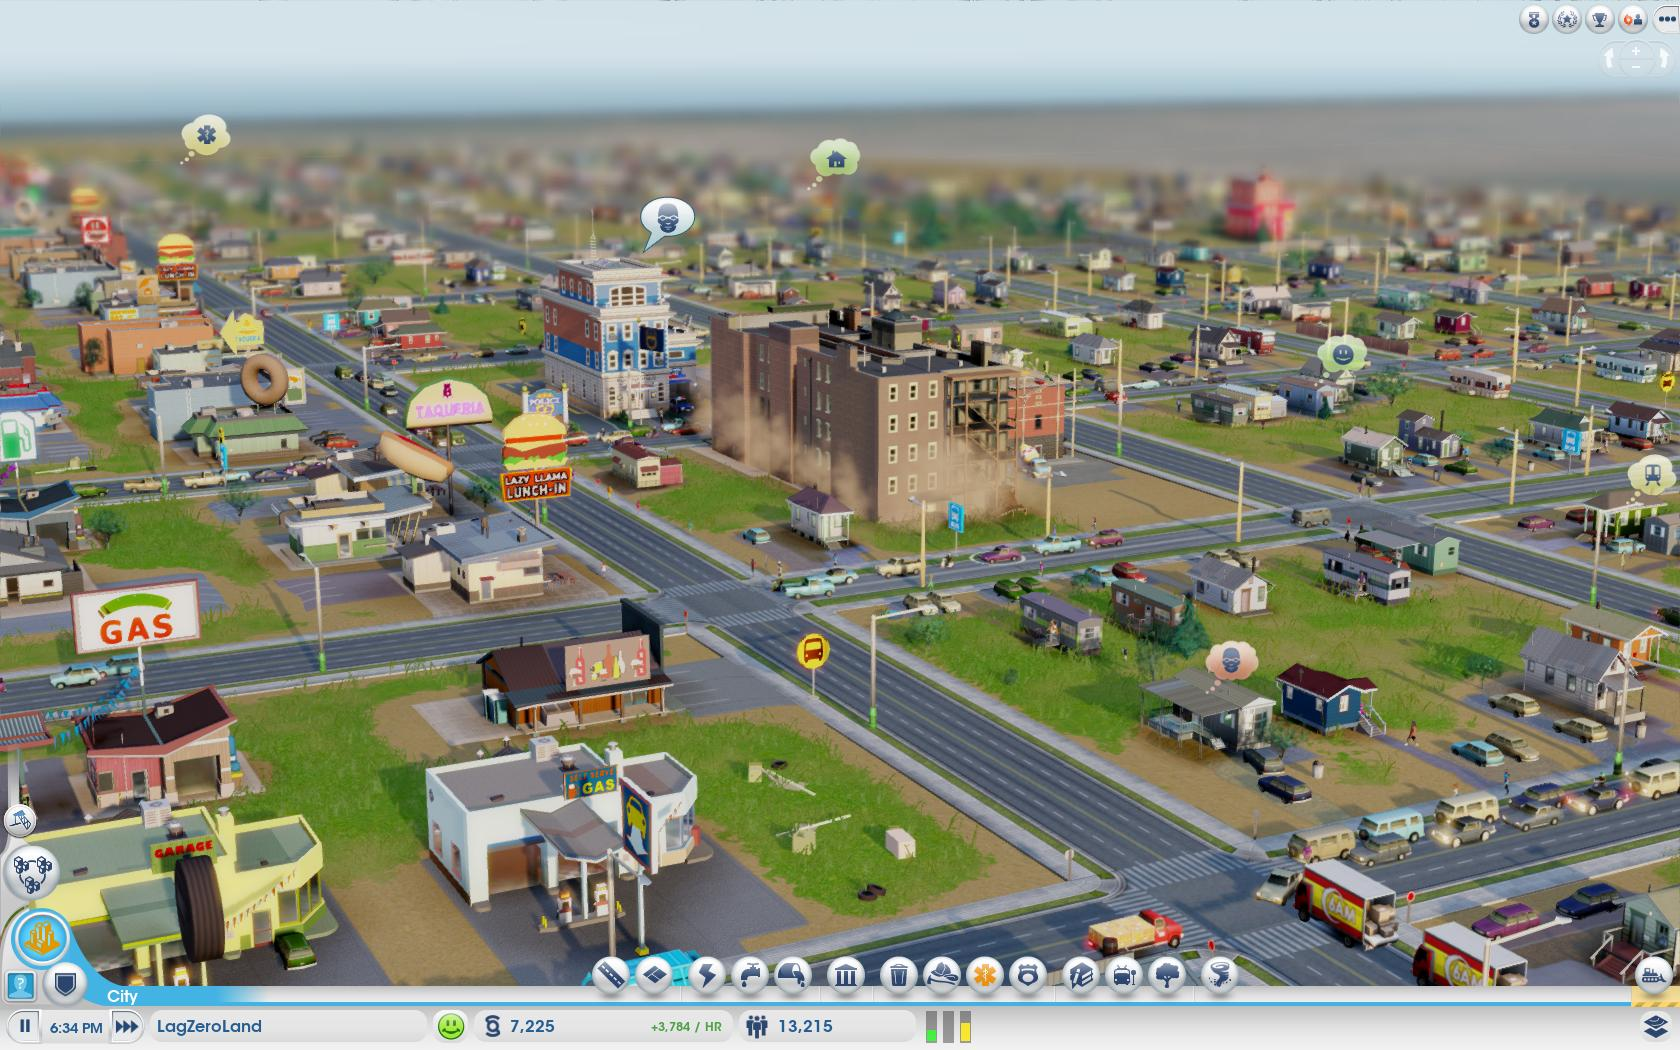
\includegraphics[height=12em]{images/SimCity}
	\label{fig:simcity}
	\caption{Pantalla del juego SimCity\texttrademark}
\end{figure}

\newpage

Otro título dentro de este género es \cities~ \footnote{https://www.citiesskylines.com/}, desarrollado por la productora finlandesa Colossal Order, y publicado por la editorial de videojuegos indie Paradox Interactive AB. Pertenece a la serie de Cities in Motion\textcopyright. Una de sus principales bazas con respecto a otros de su género es la simulación realista de tráfico, poniendo el foco en un sistema para entender los problemas en el diseño de la ciudad, y el uso de sistemas de transporte público para remediar problemas de congestión, que se ven potenciados en distintas expansiones del juego. Otra gran baza es que es altamente personalizable, pudiendo agregar desde mapas (Figura \ref{fig:cities}) hasta modelos de objetos realistas, como edificios que existen en la realidad, coches de marcas conocidas, etc. Esto hace que esté entre el top 10 de títulos con más contenido creado por la comunidad del Workshop de Steam~ \footnote{https://steamcommunity.com/app/255710/workshop}, la plataforma por referencia de compra de videojuegos en formato digital. En este proyecto vamos a utilizar esta característica de este título para poder crear un añadido que nos permita ejecutar nuestro programa lógico dentro del videojuego, y publicarlo posteriormente en Steam.

\begin{figure}[h]
	\centering
	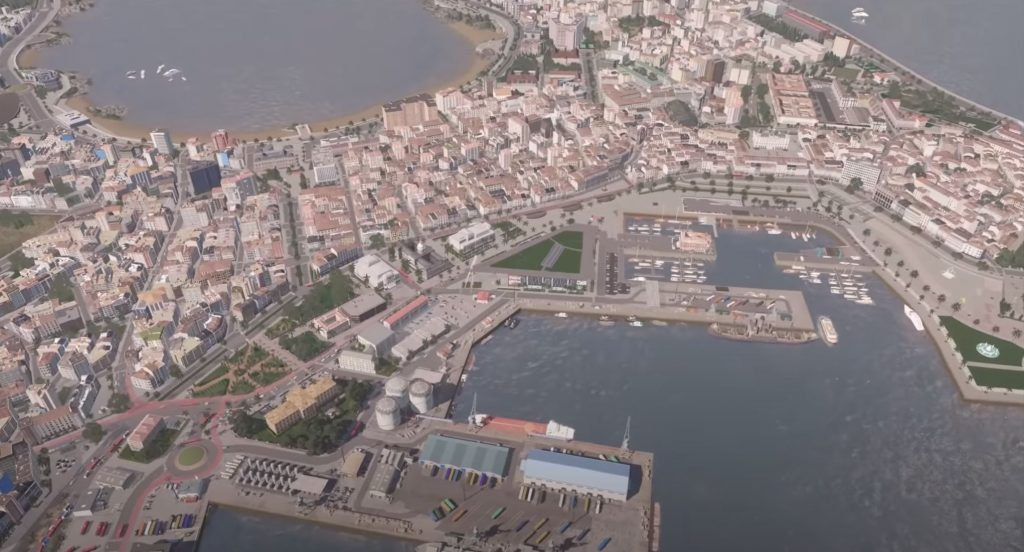
\includegraphics[height=12em]{images/CitiesCoruna}
	\label{fig:cities}
	\caption{Recreación de A Coruña en \cities}
\end{figure}

\section{Tecnologías}

Debido a las exigencias a la hora de desarrollar el proyecto, se ha optado por elegir un lenguaje de programación lógico sobre el que realizar la base declarativa del proyecto, ya que nos permitirá expresar las reglas de generación del mapa de forma matemática. También se ha escogido un segundo lenguaje multipropósito que nos permitirá desarrollar el plug-in que conectará nuestro programa lógico con el videojuego en cuestión.

\subsection{Answer Set Programming}\label{subsec:asp}

\asp (ASP) es un paradigma enfocado a la resolución declarativa de problemas difíciles, combinando un lenguaje simple con el que modelar los problemas lógicos y herramientas de alto rendimiento para la resolución de estos. \asp está basado en \emph{modelos estables}~ \cite{stablemodels}, una semántica declarativa para programas lógicos con negación. A esto se añade a que incorpora razonamiento no monótono \cite{nonmonotonic}, que permite reglas que actúan por defecto, es decir, en ausencia de información. Con esto, \asp permite resolver problemas \textit{NP-hard} de forma uniforme. \\

Una regla de programación lógica tiene el siguiente aspecto:
\begin{equation}
	\underbrace{p}_{\text{\normalsize Cabeza}} \leftarrow \underbrace{q_1, \dotsc, q_m , \textit{not } q_{m+1} ,\dotsc, \textit{not } q_n}_{\text{\normalsize Cuerpo}}.
\end{equation}

\hspace{1em}
\noindent o, en formato texto:

\begin{lstlisting}[label=lst:qreached]
      p :- q1, ... , qm, not qm1, ..., not qn.
\end{lstlisting}
en donde $p$ y todos los $q_i$ son átomos, que son los elementos que pueden ser ciertos o falsos y los literales pueden ser tanto un átomo $s$ como su negación ($\text{not } s$). Intuitivamente, una regla establece una justificación para derivar que $p$ es verdad \textit{si} todos sus átomos a la derecha de la flecha $\leftarrow$ son ciertos. Por ejemplo, si suponemos la regla

\begin{equation}\label{eq:light}
	\textit{light\_on} \leftarrow \textit{power\_on}, \textit{not } broken.
\end{equation}
informalmente significa que se puede afirmar que la luz está encendida si se puede establecer que hay electricidad y no hay razón para pensar que la lámpara esté rota. Pueden existir reglas que no tengan cuerpo,  como por ejemplo:

\begin{equation}\label{eq:power}
	\textit{power\_on} \leftarrow.
\end{equation}
Estas reglas se llaman hechos, ya que la cabeza es incondicionalmente cierta. Cuando es así, normalmente se omite la flecha $\leftarrow$. Los programas lógicos son una colección finita de reglas, en donde se expresa la ``justificación'' de un conjunto de átomos que pueden ser establecidos. Es importante señalar que \textit{not} no es el operador estándar de negación ($\lnot$), si no que significa que algo ``no es derivable''. Esto es lo que se llama negación por defecto \cite{negation}. Pensando en las dos reglas presentadas en \ref{eq:light} y \ref{eq:power}, \textit{power\_on} se puede derivar ya que es un hecho (\ref{eq:light}), mientras que \textit{broken} no porque no hay ninguna regla que lo derive. Esto nos permite derivar \textit{light\_on} (\ref{eq:power}), el cual sería el modelo estable. \\

Existe otro tipo de reglas, las cuales no tienen cabeza, es decir,
\begin{equation}
	\leftarrow B.
\end{equation}
Estas reglas se llaman \textit{constraints} o restricciones, y sirven para indicar que se desea \emph{rechazar} aquellos modelos estables en los que \textit{B} sea cierto. Asimismo, es común que programas lógicos contengan el par de reglas

\begin{align}
	a &\leftarrow B, \textit{not } \bar{a}.\\
	\bar{a} &\leftarrow B, \textit{not } a.
\end{align}
en donde $\bar{a}$ es un átomo auxiliar y B es una conjunción de literales. Esta regla aparece cuando se quiere referir tanto a un átomo \textit{a} como a su negación (estándar). Para representar este último, se introduce el nuevo átomo $\bar{a}$ y se incluye las dos reglas. Intuitivamente el rol de las reglas es seleccionar (de modo no determinista) uno de esos dos átomos en caso de que \textit{B} se satisfaga. Cuando sólo nos interesa el átomo $a$, estas reglas se pueden escribir como una regla \textit{choice} de la forma
\begin{align}
	\{a\} \leftarrow B.
\end{align}

En resumen, el paradigma de \asp se reduce al cómputo de los modelos estables de un programa lógico dado, lo cual se hace mediante herramientas llamadas \textit{solvers}, que se encargan de utilizar diferentes técnicas para obtener un modelo estable final. \\

En problemas prácticos, las reglas se aplican de forma genérica a distintos tipos de elementos o individuos. Para ello, se usan variables lógicas que son una abreviatura de los elementos a los que afecta la regla. Un programa en el que no aparecen variables se denomina programa \emph{ground}. Es por eso que, antes de resolver el programa, se usa unas herramientas llamadas \textit{grounders}, que permiten transformar el programa con variables a un programa ground. En la Figura \ref{fig:asp} se muestra el ciclo de ejecución de un programa \asp. \\

\begin{figure}[h]
	\centering
	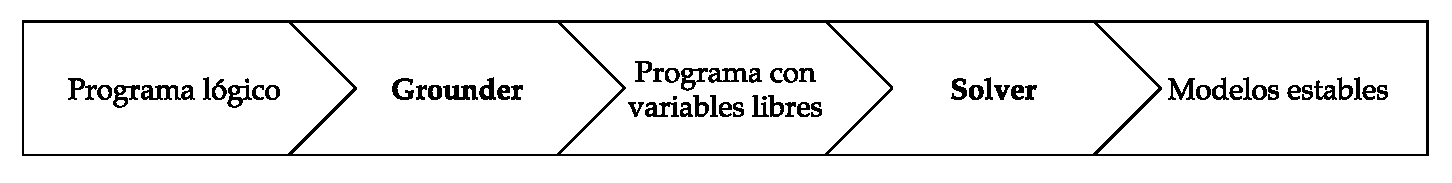
\includegraphics[height=4em]{images/ejecucion-asp}
	\label{fig:asp}
	\caption{Ejemplo de ejecución de \asp}
\end{figure}

Unas de las herramientas más importantes de \asp son las de la suite Potassco~\footnote{http://potassco.org}, un conjunto de herramientas para \asp desarrolladas en la Universidad de Postdam. Contienen las herramientas fundamentales como un grounder llamado \texttt{gringo}; un solver que es \texttt{clasp}; y una herramienta que aglutina todo el sistema \asp, \clingo. Asimismo, añade más funcionalidades al lenguaje \asp, como puede ser al resolución iterativa, debido a que permite embeber otros lenguajes como Lua o Python, que pueden interactuar con el programa escrito en \asp mediante la interfaz o \textit{API built-in} de \clingo.

\subsection{.NET Framework}

.NET Framework~~ \footnote{https://dotnet.microsoft.com/download/dotnet-framework} es un Framework o entorno de desarrollo publicado por Microsoft para el sistema operativo Microsoft Windows. El software diseñado para ser ejecutado en .NET Framework está escrito en \textit{Common Intermediate Language} o CIL, que es ejecutado en una entorno virtual llamado \textit{Common Language Runtime}, tal y como se muestra en la Figura \ref{fig:cli}. Esta máquina virtual implementa técnicas de recolección de memoria, seguridad y manejo de hilos de ejecución, además de que el software es compilado a código máquina en tiempo de ejecución, obteniendo un mejor rendimiento que otros sistemas con máquina virtual como Java, en donde la implementación de referencia cuenta con una máquina virtual basada en stack. \\

\begin{figure}[h]
	\centering
	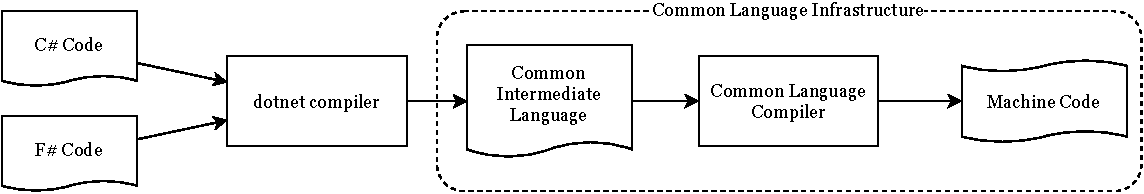
\includegraphics[height=6em]{images/arquitectura-cli}
	\label{fig:cli}
	\caption{Arquitectura de .NET Framework}
\end{figure}

Uno de los principios de este Framework es que es independiente del lenguaje de programación usado, pudiéndose programar en C/C++, Java, C\#, F\# o J\#. Estos tres últimos lenguajes también han sido diseñados por Microsoft, y fueron creados dentro del estándar de .NET Framework para cubrir diferentes necesidades (lenguaje imperativo y funcional en cada uno de los dos primeros casos, y una reimplementación del lenguaje Java en el último caso). En este proyecto usaremos en especial el lenguaje de programación C\#, ya que al ser principalmente un lenguaje imperativo y de propósito general, nos permitirá desarrollar todo el código de este proyecto. \\

Debido a que .NET Framework es un entorno solo disponible para el sistema operativo Microsoft Windows, salieron varios proyectos que se ofrecen como alternativa para ser multiplataforma, entre los cuales están CrossNet, DotGNU\footnote{http://www.dotgnu.org/}, o Mono~ \footnote{https://www.mono-project.com/}. En la actualidad el proyecto más usado es este último, que es desarrollado por el programador Miguel de Icaza, conocido por crear los proyectos GNOME y Xamarin (de la cual parte Mono). Es por eso que muchos proyectos que usan como lenguaje de programación C\# y que quieren ser multiplataforma se basan en Mono y no en .NET Framework. Uno de ellos es el motor de desarrollo de videojuegos Unity, que es uno de los más importantes en la actualidad, y, en nuestro caso, sobre el que está programado \cities. Cabe destacar que en los últimos años, Microsoft desarrolló un Framework multiplataforma y de código abierto llamado .NET Core~ \footnote{https://dotnet.microsoft.com/download/dotnet} que implementa todas las características principales de .NET Framework. A partir de Noviembre de 2020 pasó a llamarse .NET, siendo este último el sucesor de .NET Framework. \\

Otra de las características de .NET Framework que nos servirán para este proyecto es la posibilidad de manejar código nativo (bibliotecas compiladas a código máquina) con código escrito en C\#. Esto nos ha servido a la hora de poder usar las herramientas de Potassco, tal y como comentamos en la sección \ref{subsec:arquitectura}; ya que estas herramientas están escritas en C/C++, y en la actualidad no hay ninguna biblioteca que nos permita usarlas en código escrito para C\#.

\section{Herramientas}

Aparte de las tecnologías usadas para la construcción del proyecto, se han usado distintas herramientas que nos han servido a la hora de elaborar y desarrollar el sistema planteado.

\subsection{Microsoft Visual Studio}

Microsoft Visual Studio~ \footnote{https://visualstudio.microsoft.com/es} es un Entorno de Desarrollo Integrado o IDE creado por Microsoft y disponible solo para el sistema operativo Microsoft Windows. Fue pensado en su inicio para desarrollar con las tecnologías Visual de Microsoft, que son Visual C++, Visual J++ o Visual Basic, pero finalmente se ha convertido en el IDE de facto para desarrollar en las tecnologías .NET. Implementa tecnologías de autocompletado inteligente (IntelliSense\texttrademark), así como de desarrollo de software (Azure DevOps mediante un plugin llamado Team Explorer), depuración de código, despliegue de sistemas basados en web, herramientas para el diseño de interfaces gráficas y diseño de esquemas de base de datos. Incluido a esto, se puede extender las funcionalidades de Microsot Visual Studio mediante \textit{plug-ins}, que están escritos en CIL, y que se puedes descargar desde Visual Studio Galery (un repositorio centralizado de Microsoft). \\

Existen varias versiones de este editor: Enterprise, que está pensada para empresas que necesiten el despliegue en varios equipos; Professional, que está pensada para grupos con hasta 5 equipos; y Community, que solo permite una licencia única y es la gratuita. Además, existe una versión gratuita, de código libre y multiplataforma llamada Visual Studio Code, que está basado en Electron, un Frameworkd para crear aplicaciones nativas con tecnologías Web. \\

Es debido a la fuerte integración que tiene con las tecnologías .NET, y que tanto .NET Framework como Microsoft Visual Studio está disponible en Microsoft Windows; que usaremos este IDE como una de las herramientas principales para el desarrollo de este proyecto.

\subsection{Git}

Git~ \footnote{https://git-scm.com} es un sistema de control de versiones distribuido y de código abierto creado para la gestión de código fuente y desarrollo de software. Fue creado por Linus Trovalds como una alternativa libre y gratuita a BitKeeper para el desarrollo del kernel Linux por la comunidad. Está enfocado en la rapidez y eficiencia al procesar proyectos grandes, la integridad de datos, la seguridad mediante autenticación criptográfica y el fuerte soporte de un flujo de trabajo no lineal y distribuido. \\

Debido a estas características, \textit{Git} es uno de los sistemas de control de versiones más importantes hoy en día, por lo que ha permitido que existan servicios de alojamiento en linea que incluyen esta herramienta:

\begin{itemize}
	\item GitLab\footnote{https://gitlab.com}, creado por dos programadores ucranianos y que hoy en día es gestionado por GitLab Inc. Es usado por organizaciones como Sony, IBM, NASA, CERN o GNOME Foundation. Permite realizar gratuitamente repositorios privados, gestionar grupos y realizar rastreo de \textit{issues} y funcionalidades de CI/CD.
	\item Phabricator\footnote{https://www.phacility.com}, creado por Facebook como herramienta interna que integra también Mercurial y Subversion. Actualmente es de código abierto y lo usan empresas como Blender, Cisco Systems, Dropbox o KDE.
	\item Bitbucket\footnote{https://bitbucket.org}, creado por Atlassian. Este sistema integra Mercurial desde sus inicios y Git desde 2011, y está pensado para ser integrado con el resto de productos como Atlassian como Jira, Confluence y Bamboo.
	\item GitHub\footnote{https://www.github.com}, creado por tres estudiantes estadounidenses, hoy en día es gestionado por GitHub Inc. empresa que fue adquirida por Microsoft en 2018. Permite realizar rastreo de \textit{bugs}, wikis, gestión de tareas y petición de funcionalidades. Es usado por empresas como Microsoft, Google, Travis CI, Bitnami, DigitalOcean y Unreal Engine. Con la popularidad de GitHub nacieron varios servicios, como el Education Program, que permite a estudiantes el acceso gratuito a herramientas de GitHub y de partners; Gist, que permite usar GitHub como un hosting de \textit{snippets}; GitHub Marketplace, que permite comprar servicios con los que aumentar las funcionalidades en los proyectos y que muchos de ellos son gestionados por partners; y GitHub Actions, un sistema de automatización de integración continua (CI) y desarrollo continuo (CD) para construir, lanzar test y desplegar proyectos dentro de GitHub.
\end{itemize}

Nosotros usaremos este último servicio como servidor de control de versiones y para montar el sistema de automatización \textit{CI/CD}.
	\cleardoublepage

	\hypertarget{mainwork}{\chapter{Trabajo desarrollado}}
	\label{mainwork}
	En este capítulo se detalla cada uno de los puntos llevados a cabo para la realización de este proyecto, empezando por definir la propuesta realizada, luego explicar el proceso ingenieril llevado a cabo y terminar desglosando el trazado de la ejecución de este proyecto.

\section{Propuesta}

El trabajo propuesto tiene como objetivo la creación de un elemento software funcional que, usando el paradigma lógico explicado en la Sección \ref{subsec:asp}, permita la generación de un área que contenga una planificación de un polígono industrial que pueda ser generado y jugado dentro del mapa de \cities. Así mismo incluirá una interfaz gráfica interactuable que permitan al usuario marcar que zonas del terreno deben generarse y cuales no, indicando su contenido antes de lanzar el proceso de generación. \\

Antes de proceder a explicar como se ha llevado a cabo, procederemos a explicar como funciona la industria en \cities.

\subsubsection{Definición de Industria}
\label{subsubsec:terrain}

Una de las principales mecánicas en \cities es la de crear zonas de los diferentes tipos de edificios que se construir en las zonas adyacentes a las carreteras, tal y como se muestra en la Figura \ref{fig:zoneo}. Estas zonas se dividen en una cuadrícula de 5 de ancho a lo largo de la carretera, en donde cada celda es de 8x8 metros. En estas zonas se pueden definir los siguientes tipos descritos a continuación.

\begin{figure}[!h]
	\centering
	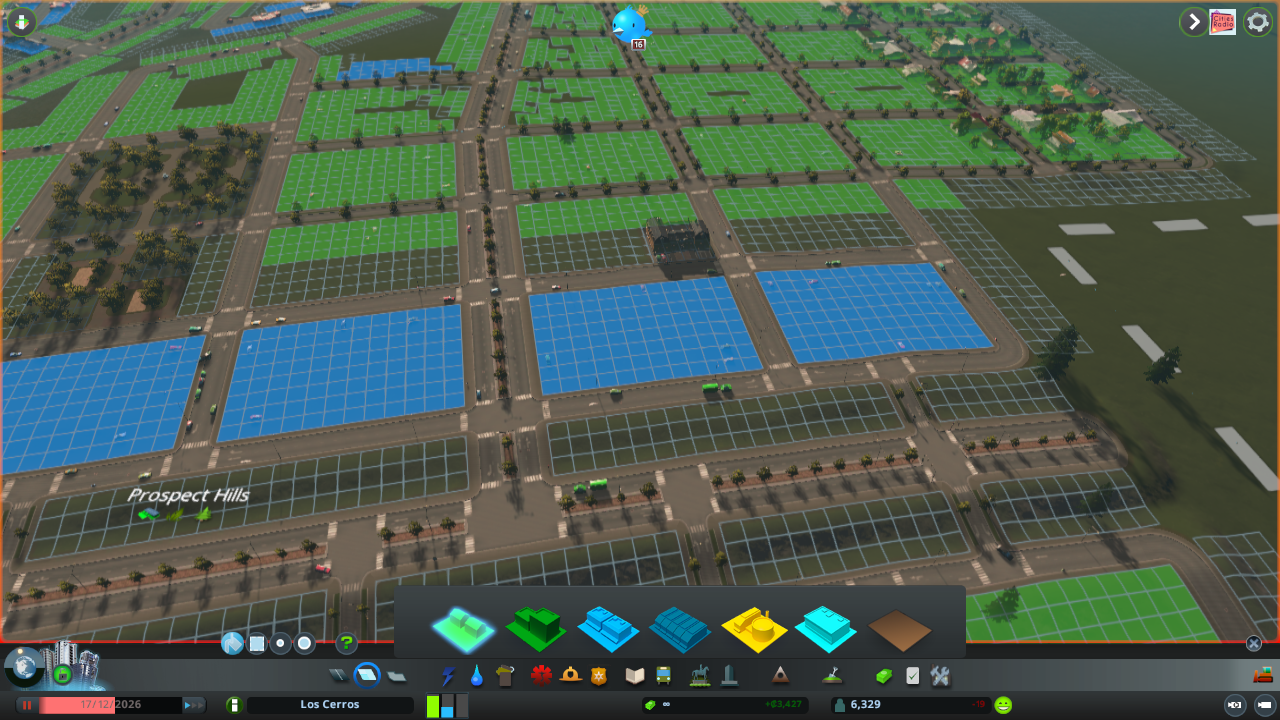
\includegraphics[width=\textwidth]{images/zoneo}
	\caption{Ejemplo de definición de zonas. En la azul las zonas comerciales y en verde las residenciales.}
	\label{fig:zoneo}
\end{figure}

\begin{itemize}
	\item \textbf{Residencial}: Corresponde a las casas donde la gente vivirá.
	\item \textbf{Comercial}: Se refiere a las tiendas y otros servicios que venden los productos creados por la industria o que son exportados.
	\item \textbf{Industrial}: Las zonas industriales proveen trabajo a los ciudadanos y crean los productos de consumo para los edificios comerciales.
	\item \textbf{Oficinas}: Las zonas de oficina dan trabajo solo a ciudadanos con alto nivel de estudios. Además no producen ni contaminación, ni tráfico, ni productos de consumo.
	\item \textbf{Servicios}: En esta categoría entran los edificios que no se pueden crear mediante zonas, si no que se fijan su construcción. Pertenecen al gobierno y dan servicios a los ciudadanos, como parques, cuarteles de policía, estaciones de buses, etc.
\end{itemize}

En este proyecto nos centraremos en las zonas industriales. Son una de las zonas que aumentan el tráfico intensamente, por lo que su planificación debe ser rigurosa. Las zonas industriales se dividen en varios tipos dependiendo de los recursos naturales que puedan usar, que pueden ser renovables (suelo fértil) o no renovables (petroleo y minerales).

\begin{itemize}
	\item \textbf{Genérica}: No tiene una especialización, por lo que corresponde a edificios genéricos. Es una de las más contaminantes pero es la base de la cadena de suministro en \cities. Proveen de trabajos para personas de estudios bajos.
	\item \textbf{Granjas}: Necesitan de suelo fértil (que es renovable) para producir recursos sin producir contaminación. Solo da trabajo para ciudadanos con nivel de estudios bajo.
	\item \textbf{Bosques}: No contamina el suelo pero genera un nivel de ruido significante. Consume también más electricidad que la industria genérica. También da trabajo para gente con nivel de estudios bajo.
	\item \textbf{Petróquímica}: Usa el suelo que contiene petróleo (que no es renovable) para producir combustible. Genera ingresos por impuestos altos, así como altos niveles de polución y consumo alto de energía.
	\item \textbf{Minera}: Usa zonas con minerales (recurso no renovable) para producir carbón. Produce menos polución e ingresos que la petroquímica pero usa más energía que la industria genérica.
\end{itemize}

\begin{figure}[!h]
	\centering
	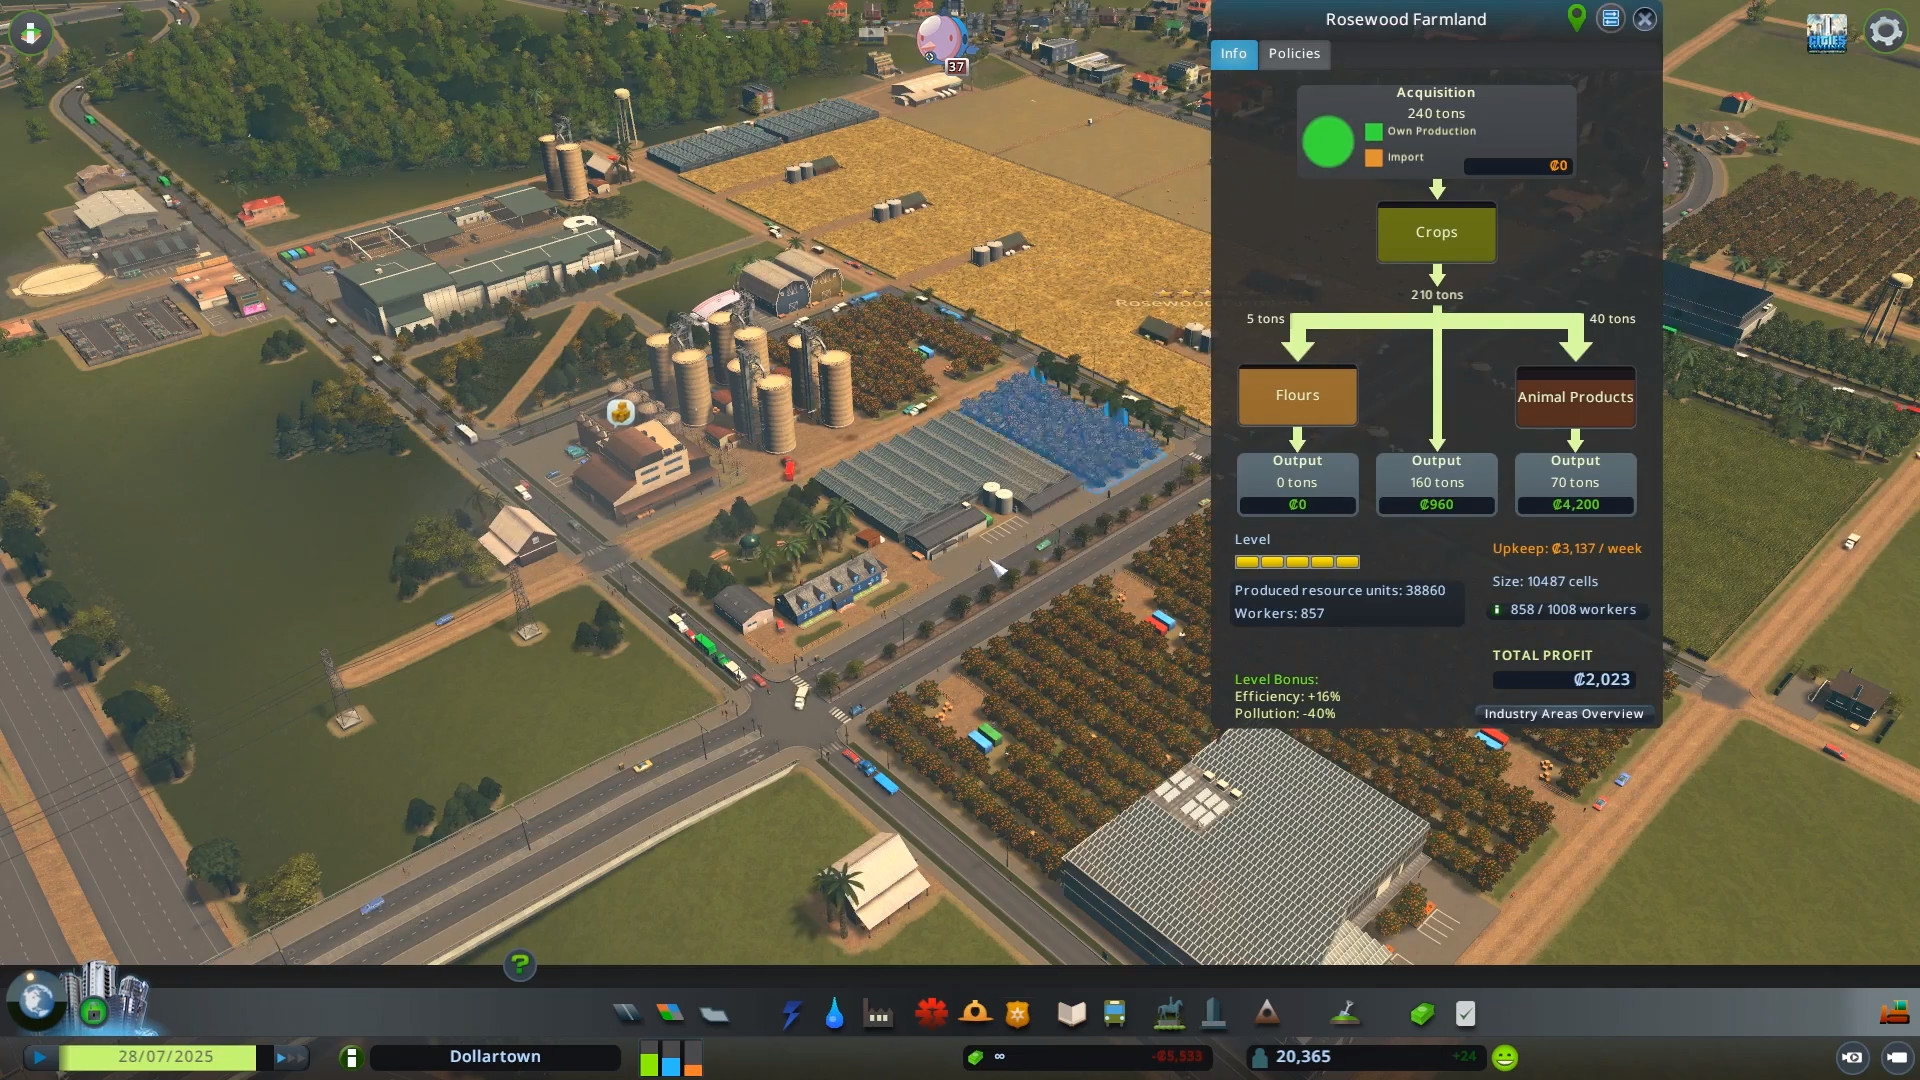
\includegraphics[width=\textwidth]{images/industries}
	\caption{Interfaz de gestión de recursos de la expansión \textit{Industries}}
	\label{fig:industry}
\end{figure}


Desde el lanzamiento de la expansión \textit{Industries}, se agregó un sistema producción, en donde se pueden procesar los recursos naturales hasta obtener productos de consumo de lujo. Para ello existen cinco tipos de edificios: extractores, procesadores, factorías, auxiliares y almacenes. Los edificios auxiliares dan zonas para que los trabajadores vivan y ofrecen mantenimiento, mientras que los almacenes sirven para guardar cada uno de los productos de cada una de las etapas.

Además, desde la expansión de \textit{Sunset Harbor} existe la industria pesquera, que agrega como recurso natural el pescado. Siguiendo el sistema de producción agregado en \textit{Industries}, este se puede procesar hasta obtener productos de consumo que se puedan exportar o vender en comercios. Dependiendo de la profundidad y el flujo del agua, se generará uno de los cuatro tipos de pescados: anchoas, atún, salmón y marisco. La polución en el agua provoca que desaparezcan este recurso del agua.

\section{Proceso de ingeniería}

En este capítulo se explica el proceso que se ha seguido para realizar el proyecto descrito. Se empezará explicando la metodología de desarrollo escogida y a continuación se expondrá y se desgranará la gestión de este trabajo.

\subsection{Metodología de desarrollo}
\label{subsec:metodologia}

A pesar de que en un primer se ha pensado que para la planificación de este proyecto se usaría la metodología de desarrollo SCRUM\cite{Schwaber:2001:ASD:559553}\cite{Schwaber:2004:APM:984028}, finalmente se ha optado por usar una amalgama entre distintas metodologías de desarrollo en espiral. Esto es debido a que SCRUM tiene unas características básicas que no se han tenido en cuenta a la hora de diseñar y desarrollar el proyecto, por lo que no sería correcto decir que se ha utilizado este tipo de metodología ágil:

\begin{itemize}
	\item \textbf{Flujo de trabajo}: El trabajo se divide en varias iteraciones entre una y cuatro semanas llamadas \textit{Sprint}, en donde en cada una de ellas se obtiene un incremento funcional del producto. Al comienzo de cada iteración se realiza una reunión en donde se identifican las tareas a realizar en esa iteración, realizando una estimación de todas; durante la realización de la iteración se realiza cada día una pequeña reunión en donde se comunica el estado actual; y, al finalizar una iteración se realiza una reunión que sirve como retrospectiva y alimentación para la próxima iteración.
	
	A la hora de realizar este proyecto, a pesar de que se ha dividido en varias iteraciones, realizando una reunión al principio de estos, y en cada iteración se finaliza con un producto funcional, el resto de elementos de la metodología SCRUM no se han llevado a cabo en la práctica.
	
	\item \textbf{Gestión de riesgos}: Uno de lo puntos de desarrollo con una metodología ágil es la de mantener una gestión de temprana de riesgos para evitar una gran desviación de la planificación. Esto se realiza mediante un panel que presenta listado ordenado de las tareas a realizar en el desarrollo total del proyecto, llamado \textit{Product backlog}. Estas tareas son las que estiman su duración y se incluyen en otro listado de tareas a realizar en cada iteración, llamado \textit{Sprint backlog}. Con esto se puede obtener una gráfica de evolución del proyecto llamado \textit{Burn down chart}, pudiendo detectar desviaciones y sobreasignaciones de forma visual debido a que también se marca el trabajo ideal de proyecto.
	
	Para este proyecto no se ha usado un desarrollo en Sprint porque no se ha realizado un seguimiento exhaustivo del mismo. En el caso de gestión de riesgos se ha usado el Product backlog como backlog de historias para hacer, sin hacer estimación.
\end{itemize}

Debido a todos estos factores expuestos, se podría indicar que la metodología usada finalmente está más cerca de una metodología basada en kanbanflow, en donde las tareas del product backlog se mueven a un tablero con columnas según el estado de la tarea; o una basada en modelos de prototipos, en donde se tiene en cuenta que cada prototipo resultante de una iteración es un modelo funcional del mismo, y en donde es revisado en la reunión de la siguiente iteración sin estar presente el cliente final, si no que solo con el director del proyecto. También en esta reunión se definen las tareas a realizar para el desarrollo del proyecto de cara a la nueva iteración.

\subsection{Gestión del proyecto}
\label{subsec:gestion}

A continuación se describirá la planificación llevada a cabo para la realización del proyecto, así como el coste y los recursos necesarios para la construcción del mismo.

\subsubsection{Planificación}

Volviendo a lo comentado en la Sección \ref{subsec:metodologia}, para la planificación se ha usado una metodología más parecida a un kanbanflow o un modelo de prototipos, dividiendo en varias tareas incrementales que, una vez terminadas, dan nuevas funcionalidades al producto final. Debido a la naturaleza del proyecto, estas tareas se han dividido en 3 épicas:

\begin{enumerate}
	\item \textbf{Generador del polígono industrial}: Las tareas presentes tienen que dar como producto final de esta épica un mod funcional para \cities. Dentro de esta épica tenemos las siguientes historias de usuario:
	\begin{enumerate}[label={\arabic*.}]
		\item \textbf{Crear prototipo de complejo industrial}: El complejo debe tener dos carreteras que se unan en la mitad con un cruce y en cada uno de los cuatro espacios se debe situar una nave.
		\item \textbf{Generar rejilla simple}: Se seleccionará una sección del mapa y se creará un conjunto de carreteras que formen una cuadrícula.
		\item \textbf{Conectan ClingoSharp con IndustryLP}: Se incluirá el proyecto ClingoSharp como dependencia de IndustryLP y se procederá a hacer una generación sencilla.
		\item \textbf{Funcionalidades extra}: Se añadirán a la selección de la región operaciones de movimiento de la región, cambio de tamaño y rotación de la misma.
		\item \textbf{Añadir restricciones/preferencias}: Para cada parcela, el usuario podrá proponer un edificio o prohibir la generación del mismo.
		\item \textbf{Establecer plantillas}: Se incluirá una lista de las distintas topologías de carreteras que el usuario podrá seleccionar, y que se usarán en vez de la cuadrícula.
		\item \textbf{Construir polígono}: Una vez seleccionado la solución de Clingo, el sistema deberá construir objetos servibles dentro del entorno de \cities.
	\end{enumerate}

	\item \textbf{Interfaz C\# con Clingo}: El resultado de esta épica es crear un producto final que sea una librería que actúe como binding de Clingo para C\#, que será usado por el mod creado en \cities:
	\begin{enumerate}[label={\arabic*.}]
		\setcounter{enumii}{7}
		\item \textbf{Generar biblioteca dinámica}: Como Clingo está escrito en C/C++, la idea es que se pueda crear una biblioteca dinámica nativa (.dll en Microsoft Windows, .so en GNU/Linux) que se pueda usar para ClingoSharp.
		\item \textbf{Cargar programa lógico sencillo}: Se deberían crear los módulos básico para poder invocar Clingo desde un programa en C\# y permitir que cargue un programa lógico.
		\item \textbf{Conectan ClingoSharp con IndustryLP}: Se incluirá el proyecto ClingoSharp como dependencia de IndustryLP y se procederá a hacer una generación sencilla.
		\item \textbf{Completar módulo Control}: El objetivo es poder leer cada uno de los átomos resultantes de un modelo estable. Además poder incorporar llamadas de forma asíncrona a Clingo.
		\item \textbf{Implementar módulo de modelos estables}: El objetivo es poder leer cada uno de los átomos resultantes de un modelo estable. Además poder incorporar llamadas de forma asíncrona a Clingo.
		\item \textbf{Añadir tests unitarios}: Se definirán los tests básico para las funcionalidades principales de Clingo.
	\end{enumerate}

	\item \textbf{Documentación}: El objetivo de esta épica es la de crear las diferentes documentaciones necesarias del proyecto. Se divide en:
	\begin{enumerate}[label={\arabic*.}]
		\setcounter{enumii}{13}
		\item \textbf{Memoria del proyecto}: Crear este documento que tendrá toda la información del proyecto.
		\item \textbf{Documentación del IndustryLP}: Generará los diagramas y la documentación de código necesaria.
		\item \textbf{Documentación de ClingoSharp}: Se crearán los diagramas y documentación del código necesaria.
	\end{enumerate}
\end{enumerate}

Considerando las tareas descritas anteriormente, en la Tabla \ref{table:dedicacion} podemos ver la dedicación en horas llevada a cabo para cada proyecto. Debido a que no se ha realizado una estimación antes de la realización, no tenemos un dato previsto, si no que es directamente el valor final tangible.

\begin{table}[!h]
	\centering
	\begin{tabular}{ c c }
		\bfseries{Tarea} & \bfseries{Tiempo (h)} \\
		\hline
		01 & 30 \\
		02 & 6 \\
		03 & 30 \\
		04 & 30 \\
		05 & 40 \\
		06 & 45 \\
		07 & 15 \\
		08 & 6 \\
		09 & 15 \\
		10 & 30 \\
		11 & 30 \\
		12 & 15 \\
		13 & 15 \\
		14 & 40 \\
		15 & 8 \\
		16 & 8 \\
		\hline
		\bfseries{Total} & 363 \\
		\hline
	\end{tabular}
	\caption{Desglose de la dedicación a las historias de usuario.}
	\label{table:dedicacion}
\end{table}

\subsubsection{Coste y recursos}

Para calcular el coste de los recursos humanos que ha supuesto este proyecto, aparte de las 363 horas totales se ha añadido un 10\% a mayores que incluye las reuniones de seguimiento por parte del director del proyecto. 

\section{Análisis del software}

Una vez definido el sistema y planificada su construcción, se ha realizado un análisis en donde se identifican los requisitos que debe cumplir el software una vez terminado el proyecto. Eso suma 37 horas al proyecto, dando un total de 400 horas total. Teniendo esto en cuenta, y siguiendo la Guía Salarial del Sector TI en Galicia \cite{guia_galicia}, se han estimado los costes que se pueden ver en la Tabla \ref{table:costehumano}.

\begin{table}[!h]
	\centering
	\begin{tabular}{ c c c c }
		\bfseries{Recurso} & \bfseries{Tiempo (h)} & \bfseries{Coste (\euro/h)} & \bfseries{Total} \\
		\hline
		Doctor Investigador & 37 & 24,00 & 888,00 \\
		Analista Programador & 363 & 9,00 & 3267,00 \\
		\hline
		\bfseries{Total} & 400 & & 4155,00 \\
		\hline
	\end{tabular}
	\caption{Coste de los recursos humanos del proyecto.}\label{table:costehumano}
\end{table}

\begin{table}[!h]
	\centering
	\begin{tabularx}{\textwidth}{ l X X X X }
		\bfseries{Recurso} & \bfseries{Vida (mes)} & \bfseries{Uso (mes)} & \bfseries{Coste (\euro)} & \bfseries{Total (\euro)} \\
		\hline
		Portátil & 48 & 10 & 800,00 & 166,67 \\
		\cities & $\infty$ & 10 & 27,99 & 27,99 \\
		Clingo & $\infty$ & 10 & - & 0 \\
		.NET Framework & $\infty$ & 10 & - & 0 \\
		Visual Studio & $\infty$ & 10 & - & 0 \\
		Github & $\infty$ & 10 & - & 0 \\
		LaTeX & $\infty$ & 10 & - & 0 \\
		\hline
		\bfseries{Total} & & & & 194,66 \\
		\hline
	\end{tabularx}
	\caption{Coste de los recursos humanos del proyecto.}\label{table:costematerial}
\end{table}

Por otro lado, en la \ref{table:costematerial} se recoge la lista de recursos materiales y lógicos necesarios para el desarrollo de este proyecto. Para el caso de los recursos \textit{hardware} se ha tenido en cuenta el tiempo de uso para este proyecto con respecto a su vida útil, mientras para los recursos \textit{software}, se ha preferido por usar herramientas y bibliotecas de uso libre y gratuitas, de ahí que el coste no esté contado para el resultado final. \\

Con todo esto se puede concluir que el coste total del proyecto asciende hasta \EUR{4349,66} en total.

\subsection{Requisitos funcionales}
\label{subsec:funcrequirements}

Los requisitos funcionales son aquellas condiciones indispensables que estipulan las funcionalidades que debe proporcional el sistema. Para este proyecto se ha recogido los diferentes requisitos:

\begin{itemize}
	\item Generación de un poligono industrial que sea legible por el videojuego \cities.
	\item Permitir añadir restricciones sobre ciertas zonas del mapa.
	\item Poder mostrar los resultados de la generación dentro del videojuego.
\end{itemize}

\subsection{Requisitos no funcionales}

Los requisitos no funcionales, por su contra, son aquellas condiciones indispensables que debe cumplir el sistema a la hora de diseñar e implementar. Para este proyecto se han tenido en cuenta estos requisitos:

\begin{itemize}
	\item Eficiencia y eficacia: El generador debe responder en el menor tiempo posible arrojando una respuesta óptima.
	\item Escalabilidad: El generador debe trabajar con mapas de diferentes tamaños, por lo que el sistema debe poder soportar cualquier tamaño de entrada.
	\item Usabilidad: La interfaz gráfica debe ser lo más sencilla posible, evitando que el usuario tenga que realizar tareas tediosas a la hora de construir mapas.
\end{itemize}

\section{Diseño del sistema}

Una vez definidos los requisitos se ha procedido a realizar el diseño software del sistema en cuestión, empezando a concretar la arquitectura propuesta y luego desarrollando los casos de uso y diagramas de clases.

\subsection{Arquitectura software}
\label{subsec:arquitectura}

Este proyecto se ha dividido en dos tipos de arquitectura dada la naturaleza del problema. Esto es debido a que estamos implementando diferentes paradigmas, y cada una tiene su forma de diseñarse. \\

\begin{figure}[!h]
	\centering
	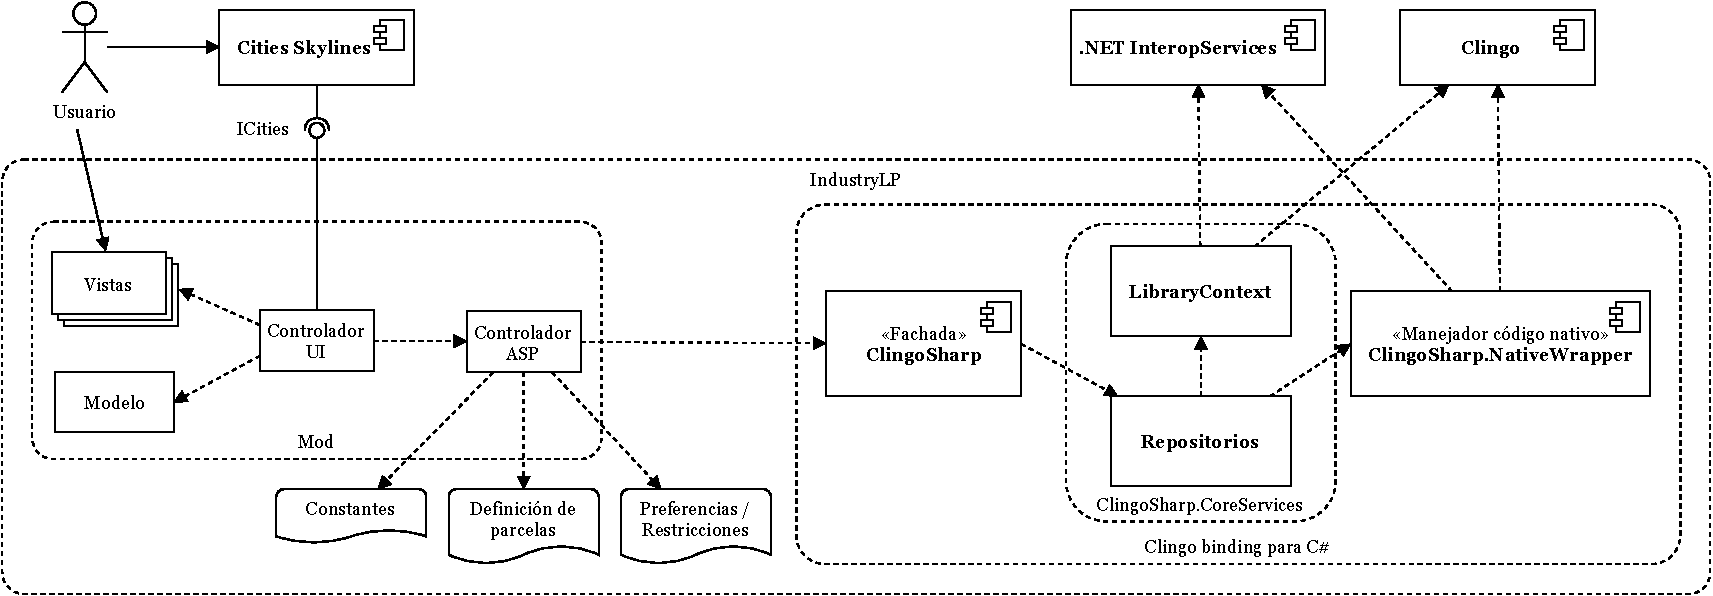
\includegraphics[width=\textwidth]{images/arquitectura-mod}
	\caption{Arquitectura del mod de \cities}
	\label{fig:arquitectura-mod}
\end{figure}

Como primera parte vamos a analizar la arquitectura del software que se ejecuta dentro de \cities. Tal y como se puede ver en la Figura \ref{fig:arquitectura-mod}, este se ha divido en dos capas para permitir sus reusabilidad en distintos proyectos. En la primera capa tendríamos la interfaz del mod en si mismo. Este se basa en una arquitectura Modelo-Vista-Controlador (MVC), en donde el controlador se encargará de reaccionar antes los eventos de las vistas, que son la parte que el usuario manipula, y modificar el modelo, que son los datos que se guardan en memoria en este caso. \\

Además, el controlador de la interfaz se conectará con el controlador del modulo ASP para hacer llamadas a Clingo y obtener el resultado de las preferencias, tal y como se explica en la Sección \ref{subsubsec:generator}. Este módulo a su vez llama a la segunda capa, que se corresponde con un \textit{binding} o adaptación de la API en C de Clingo para el lenguaje de programación C\#. Este binding usa como referencia final la API en Python de Clingo\footnote{https://potassco.org/clingo/python-api/5.4}, la cual está dividida en módulos. Es por eso que nos hemos basado en una arquitectura de repositorios, en donde hay una fachada que llama a cada una los distintos componentes, que contienen como contexto la referencia a la biblioteca de Clingo, y los cuales a su vez llaman a otro componente que se encarga de hacer la llamada a la API en C de Clingo. \\

\begin{figure}[!h]
	\centering
	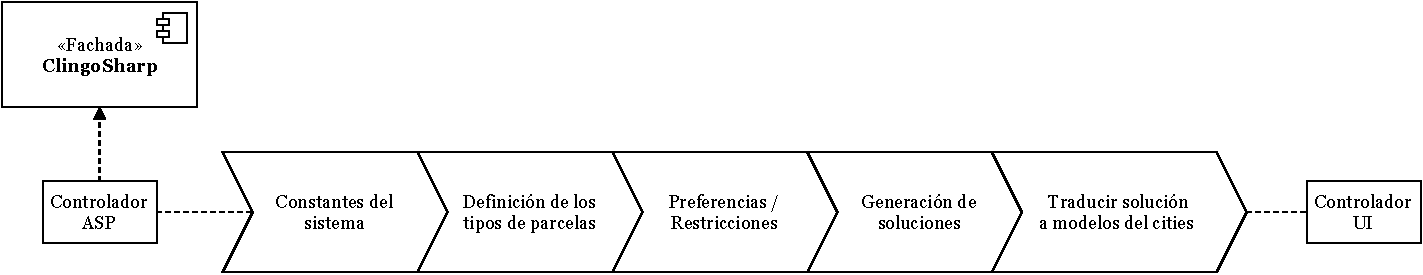
\includegraphics[width=\textwidth]{images/arquitectura-asp}
	\caption{Arquitectura del programa lógico}
	\label{fig:arquitectura-asp}
\end{figure}

En la segunda parte analizaremos la arquitectura del programa lógico. Como ya comentamos en la Sección \ref{subsec:asp}, para resolver un programa lógico necesitamos transformarlo a su equivalente con variables libres mediante un grounder, y obtener los modelos estables mediante un solver. Debido a que es un proceso de transformación se ha ideado el usar una arquitectura en \textit{pipeline}, en donde la salida de cada proceso es la entrada del siguiente. Tal y como se puede ver en la Figura \ref{fig:arquitectura-asp}, se ha divido en una etapa de definición de constantes del sistema lógico, una etapa de definición del los tipos de parcelas (obteniendo previamente la información de los modelos existentes en \cities), una etapa de preferencias o restricciones del tipo o posición de las parcelas, una etapa de obtención de los modelos estables, y una última etapa de traducción de cada átomo del modelo estable a un modelo que pueda comprender \cities. Cada una de las etapas se explicarán en la Sección \ref{subsubsec:generator}.

\subsection{Casos de uso}
\label{subsec:cases}

El sistema tiene en cuenta que se usará en todo momento por un único usuario, el cual llevará a cabo todas las funcionalidades propuestas en la Sección \ref{subsec:funcrequirements} a través de una interfaz gráfica. Estos requisistos funcionales se transforman, por tanto, en los casos de uso del sistema que se proponen en la Tabla \ref{fig:casos-uso1}

\begin{figure}[!h]
	\centering
	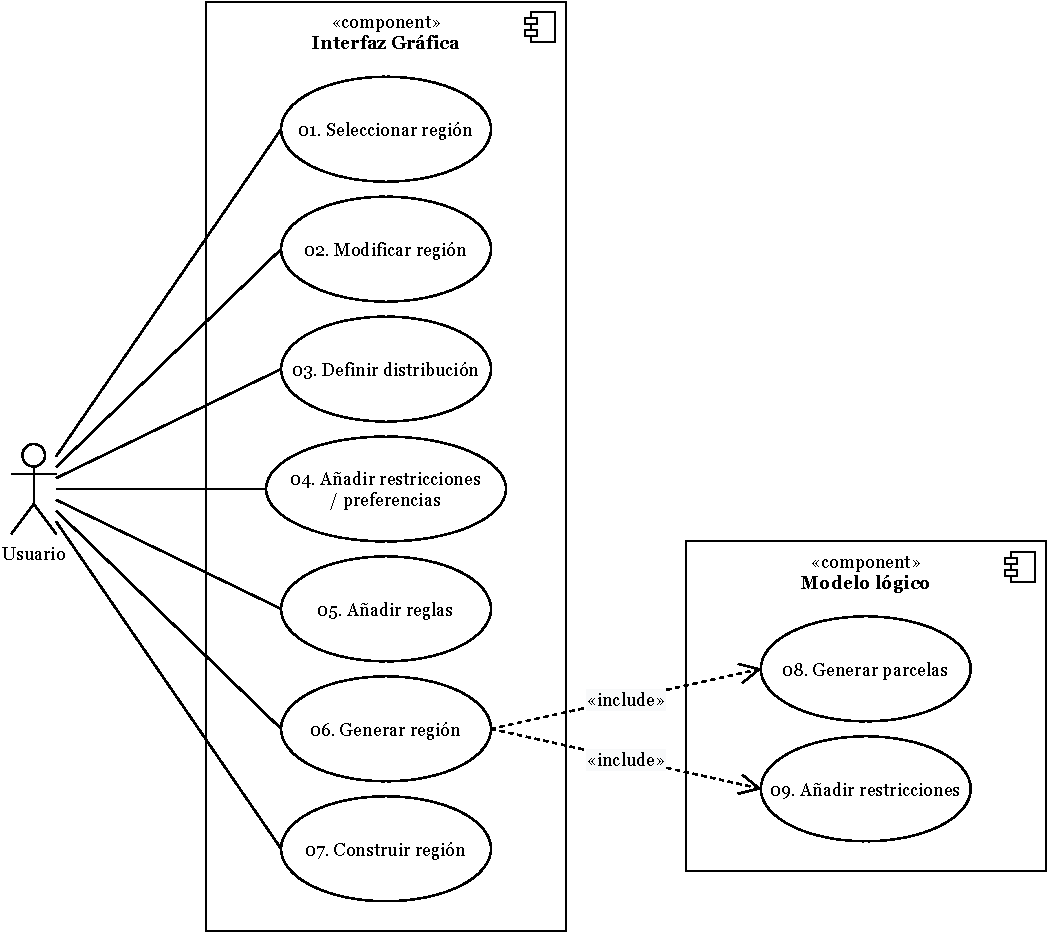
\includegraphics[width=\textwidth]{images/casos-uso}
	\caption{Diagrama de casos de uso del sistema propuesto}
	\label{fig:casos-uso}
\end{figure}

\begin{table}[!h]
	\begin{tabularx}{\textwidth}{ c c X }
		\bfseries{CU} & \bfseries{Nombre} & \bfseries{Descripción} \\
		\hline
		01 & Seleccionar región & El usuario puede pinchar en cualquier zona del mapa de \cities y marcar una región. \\
		\hline
		02 & Modificar región & Una vez marcada una región, el usuario puede cambiar el tamaño y la rotación de esta mediante movimiento del ratón. \\
		\hline
		03 & Definir distribución & Una vez establecida la región, el usuario puede indicar que tipo de topología de carreteras se va a generar en la región. \\
		\hline
	\end{tabularx}
	\caption{Descripción de casos de uso 1}
	\label{table:casos-uso1}
\end{table}

\begin{table}[!h]
	\begin{tabularx}{\textwidth}{ c c X }
		\bfseries{CU} & \bfseries{Nombre} & \bfseries{Descripción} \\
		\hline
		04 & \makecell{Añadir restricciones \\ / preferencias} & Dada una distribución, el usuario puede marcar que edificios prefiere generar y cuales quiere descartar de la generación. \\
		\hline
		05 & Añadir reglas & Antes de empezar a generar la región, el usuario puede modificar de forma opcional la generación indicando nuevas reglas escribiendolas en un campo de texto. \\
		\hline
		06 & Generar región & El sistema deberá generar una región válida y mostrarla. Para eso se apoyará de los casos de uso 08 y 09. \\
		\hline
		07 & Construir región & Una vez seleccionada la región que el usuario quiere construir, se invocará a \cities para que cree los objetos necesarios en el juego para que se pueda usar por la IA. \\
		\hline
		08 & Generar parcelas & El sistema deberá seleccionar un tipo edificio para cada tipo de parcela. \\
		\hline
		09 & Añadir restricciones & Una vez seleccionado el tipo de edificio, el sistema añadirá las restricciones de cada parcela para que el sistema lógico genere una solución que satisfaga dichas restricciones. \\
		\hline
	\end{tabularx}
	\caption{Descripción de casos de uso 2}
	\label{table:casos-uso2}
\end{table}

\subsection{Diseño del programa lógico}
\label{subsubsec:generator}

Retornando a lo comentado en la Sección \ref{subsec:arquitectura}, una de las piezas fundamentales de este proyecto es la definición de un generador de polígonos industriales en formato declarativo. Para ello usamos el paradigma de programación lógica, que usa la tecnología Answer Set Programming, tal y como se expone en la Sección \ref{subsec:asp}. \\

Con esto, el objetivo de este generador es intentar dar un modelo declarativo basado en reglas que corresponda en mayor o menor medida con la definición de un polígono industrial. A continuación explicamos el diseño de cada una de las etapas que consta el sistema de generación.

\subsubsection{Constantes del sistema lógico}

Como primer paso para la generación del polígono industrial, definimos unos átomos que nos servirán para indicar el tipo de algunas variables. En concreto hemos definido el átomo \texttt{row(X)}, que contiene la definición de cada fila, y \texttt{column(X)} que es la contraparte para columnas. En el caso de los tipos de edificio disponibles, se ha creado el átomo \texttt{str\_parcel(X)}, el cual guarda como string el nombre de cada uno de los edificios disponibles en \cities.

\subsubsection{Definición de los tipos de parcela}

Con las constantes ya definidas, se ha definido una regla para la generación de cada parcela \texttt{parcel(X, Y, B)} con una \textit{choice rule}. La \textit{choice rule} tiene cardinalidad 0 - 1, que se expresa como \textit{min \{p\} max} e indica que puede existir o no un átomo \texttt{parcel(X, Y, B)} dado un tipo de edificio \texttt{str\_parcel(B)} para cada celda \texttt{row(X), column(Y)}. \\

Con esto le decimos a Answer Set Programing que puede elegir cualquier combinación para cada parcela, incluyendo no generar una parcela de un tipo dato. Esto puede generar soluciones donde no existe parcelas, o donde para una parcela existen varias soluciones. Para restringir las soluciones a modelos estables en donde exista un solo átomo \texttt{parcel(X, Y, B)}, vamos a añadir un esquema de comprobación-restricción. Este esquema se basa en definir un átomo auxiliar que marque una comprobación concreta, y luego una restricción (una regla sin cabeza) para este átomo.

\begin{lstlisting}[caption={Código para la generación de parcelas},captionpos=b,label=lst:parcel_def]
% Generacion %
0 { parcel(X, Y, B) : str_parcel(B) } 1 :- row(X), column(Y).

% Comprobacion %
sell_parcel(X, Y) :- row(X), column(Y), str_parcel(B), parcel(X, Y, B).

% Restriccion %
:- row(X), column(Y), not sell_parcel(X, Y).
:- parcel(X, Y, S1), parcel(X, Y, S2), str_parcel(S1), str_parcel(S2), row(X), column(Y), S1 != S2.
\end{lstlisting}

En nuestro caso usaremos como átomo auxiliar \texttt{sell\_parcel(X, Y)}, que nos indicará que existe una parcela en una posición, y como restricciones definiremos una regla para que no existan celdas sin el átomo \texttt{sell\_parcel(X, Y)}, y otra regla para que no existan celdas con tipos de edificio distintos.

\subsubsection{Preferencias/Restricciones de parcelas}

Con la definición de cada parcela a una posición dada hecha, añadiremos más reglas para delimitar la generación de los modelos estables a las preferencias del usuario. Para ello, desde la interfaz podemos indicar si queremos que un edificio se genere en una posición dada, o si queremos que un edificio no se genere nunca en una posición. \\

\begin{lstlisting}[caption={Preferencias de parcelas},captionpos=b,label=lst:preference_def]
% Preferencia de colocacion de parcelas
parcel(1, 1, "Cargoyard").
parcel(2, 3, "Wind turbine").
parcel(2, 2, "Cargoyard").
parcel(3, 1, "General Factory 3x2").
        ...

% Restricciones del tipo de edificio
:- parcel(4, 1, "General Factory 2x2").
:- parcel(1, 2, "Forestry 4x4").
:- parcel(2, 2, "Forestry 4x3").
\end{lstlisting}

En la primera parte vamos a traducir las preferencias a hecho, que son los propio átomo, o también se pueden ver como reglas sin cola y actúan como valores de verdad dentro del modelo lógico. En el segundo caso, se traducirán a restricciones o reglas sin cabeza, tal y como vimos en la sección anterior. En el Listado \ref{lst:preference_def} vemos ejemplos de estas preferencias. \\

Uno de los resultados lógicos que podemos tener aquí es que el usuario ponga tanto como preferencia como restricción el mismo tipo de edificio. Aquí el resultado que nos devuelve clingo es que el modelo es insatisfactible, es decir, no existe ningún modelo estable que cumpla con el programa lógico, tal y como se muestra en la Figura \ref{fig:clingo-unsat}. \\

\begin{figure}[!h]
	\centering
	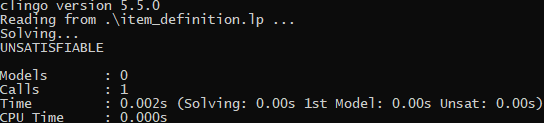
\includegraphics[width=\textwidth]{images/clingo-unsat}
	\caption{Ejemplo de un programa lógico sin solución}
	\label{fig:clingo-unsat}
\end{figure}

Otras formas de delimitar la generación es mediante las distancias y la topología de la generación. Esto nos permite hacer reglas más complejas en donde indiquemos restricciones más avanzadas, como que no queremos que dos tipos de edificios estén cerca, por ejemplo en el caso de que sea industria contaminante con industria verde. Para ello podemos usar algún algoritmo, como distancia de manhattan (tal y como se muestra en el Listado \ref{lts:manhattan_def}) o k-vecino más cercano. \\

\begin{lstlisting}[caption={Cálculo de la distancia del taxista en Aswer Set Programing},captionpos=b,label=lst:manhattan_def]
distance(S1, S2, |X1-X2|+|Y1-Y2|) :- parcel(X1, Y1, S1), parcel(X2, Y2, S2), X1 != X2, Y1 != Y2.
neighbour(S1, S2) :- distance(S1, S2, 1).
\end{lstlisting}

Para delimitar la generación con este tipo de reglas, podemos usar los átomo que acabamos de crear como una estrategia de \textit{divide y vencerás}, introduciendo estos átomos en hechos o en prohibiciones. Esto se ve reflejado en el Listado

\begin{lstlisting}[caption={Prohibiciones de generación de edificios},captionpos=b,label=lst:distance_rules]
neighbour("Forestry 3x3", "Forestry 3x2").
neighbour("Forestry 3x4", "Forestry 3x2").
neighbour("Forestry 3x3", "Forestry 3x2").

:- distance("Forestry 3x3", "Farm Village", D), D < 4.
:- distance("Forestry 3x4", "Farm Village", D), D < 4.
\end{lstlisting}

\subsection{Implementación}
\label{subsec:implementacion}

Una vez analizado el proyecto en cuestión, y explicado como funciona el programa lógico, pasaremos a detallar el diseño de los componentes principales de los sistemas creados para usar en \cities.

Primeramente empezaremos explicando como funcionan las diferentes acciones en \industrylp. Pensando en su reusabilidad, y que en un futuro el número de acciones pueda crecer, se ha pensado en implementarlas usando un patrón estrategia. Tal y como se muestra en la Figura \ref{fig:actions}, cada acción deriva de la clase \texttt{ToolAction}.

\begin{figure}[!h]
	\centering
	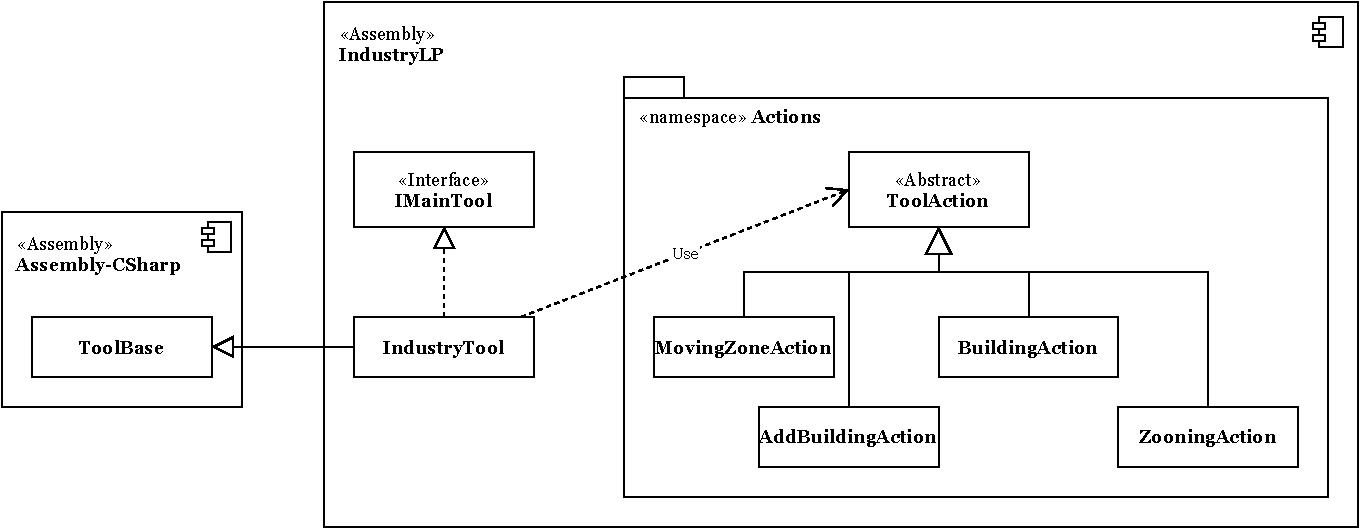
\includegraphics[width=\textwidth]{images/actions}
	\caption{Acciones de la interfaz}
	\label{fig:actions}
\end{figure}

Esta clase abstracta define una serie de métodos comunes que corresponden al ciclo de vida pensado para cada una de las acciones, representados en la Figura \ref{fig:action-lifecycle}. El ciclo de vida de una accion es controlado por la clase \texttt{IndustryTool}, que a su vez deriva de \texttt{ToolBase}, una clase abstracta que nos proporciona la interfaz de \cities y que también tiene un ciclo de vida, pero que es controlado por el propio juego.

\begin{figure}[!h]
	\centering
	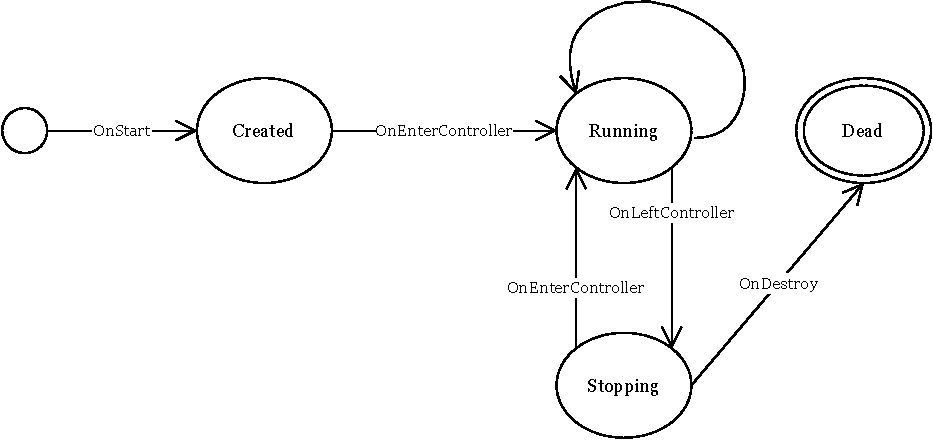
\includegraphics[width=\textwidth]{images/action-lifecycle}
	\caption{Ciclo de vida de una actividad}
	\label{fig:action-lifecycle}
\end{figure}

Es por eso que, dependiendo del estado en el que se encuentre el juego y la interfaz, la clase \texttt{IndustryTool} delegará en cada una de las acciones. Además, \texttt{IndustryTool} implementa la interfaz \texttt{IMainTool}, que define una serie de métodos que pueden usan las acciones para cambiar de estado o ejecutar otra acción, evitando así el acoplamiento entre \texttt{IndustryTool} y cada una de las acciones concretas. \\

Con respecto a la generación de distribuciones, pensando también en la reusabilidad y en la implementación de nuevas topologías de parques industriales en un futuro, también se optó por usar un patrón de diseño, en este caso de \textit{Template Method}. El diseño de la generación de distribuciones se muestra en la Figura \ref{fig:distributions}.

\begin{figure}[!h]
	\centering
	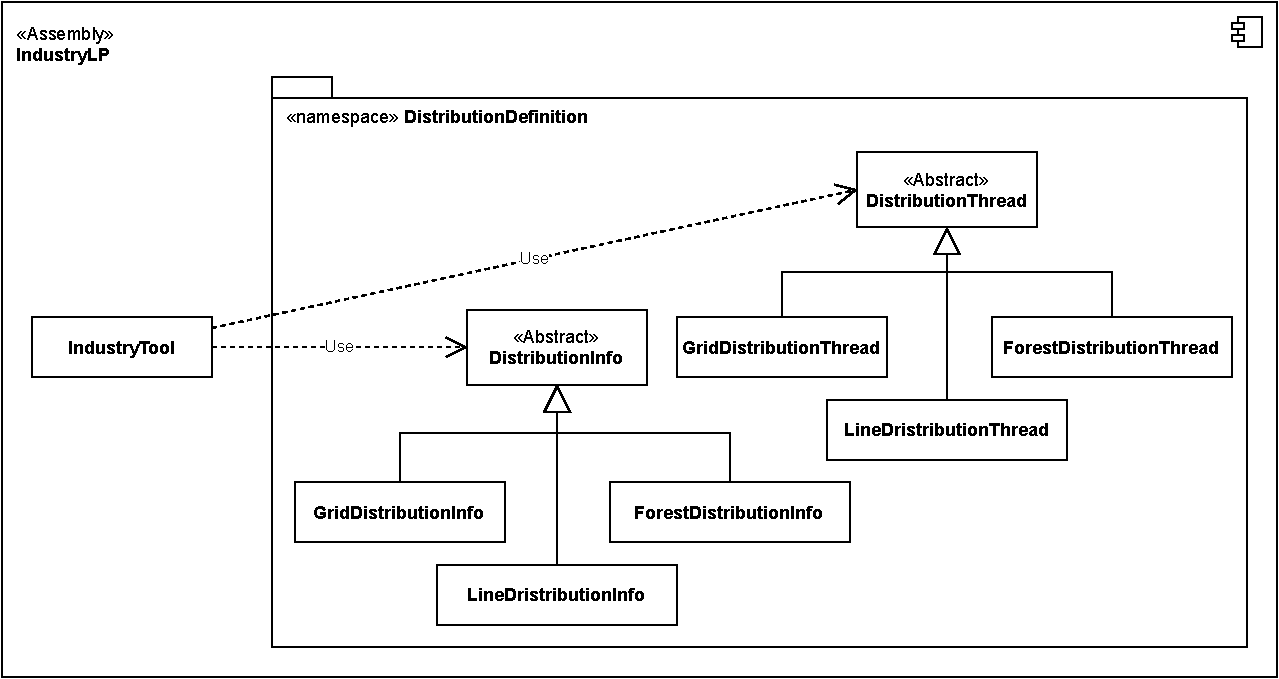
\includegraphics[width=\textwidth]{images/distribuciones}
	\caption{Definición de las distribuciones}
	\label{fig:distributions}
\end{figure}

Aquí, existen dos clases abstractas: \texttt{DistributionThread}, que define los métodos para la ejecución del algoritmo de generación de la distribución, el cual a diferencia del problema principal, este está implementado de forma imperativa; y \texttt{DistributionInfo}, que contiene la información resultante de la generación del algoritmo, y que define métodos de navegación de parcelas según la distribución. \\

En el caso del sistema que se encarga de conectar y ejecutar la biblioteca de Clingo, se ha optado por una arquitectura de tipo repositorio, tal y como se muestra en la Figura \ref{fig:clingosharp-repository}. Cada módulo de Clingo conecta con un módulo del componente \textit{ClingoSharp.NativeWrapper}, que se encargar de enlazar dinámicamente las funciones de la API en C con métodos internos de cada módulo. Estos módulos a su vez exponen funciones con tipos de datos manejados por C\# mediante interfaces, que derivan de una interfaz general llamada \texttt{IClingoModule}.

\begin{figure}[!h]
	\centering
	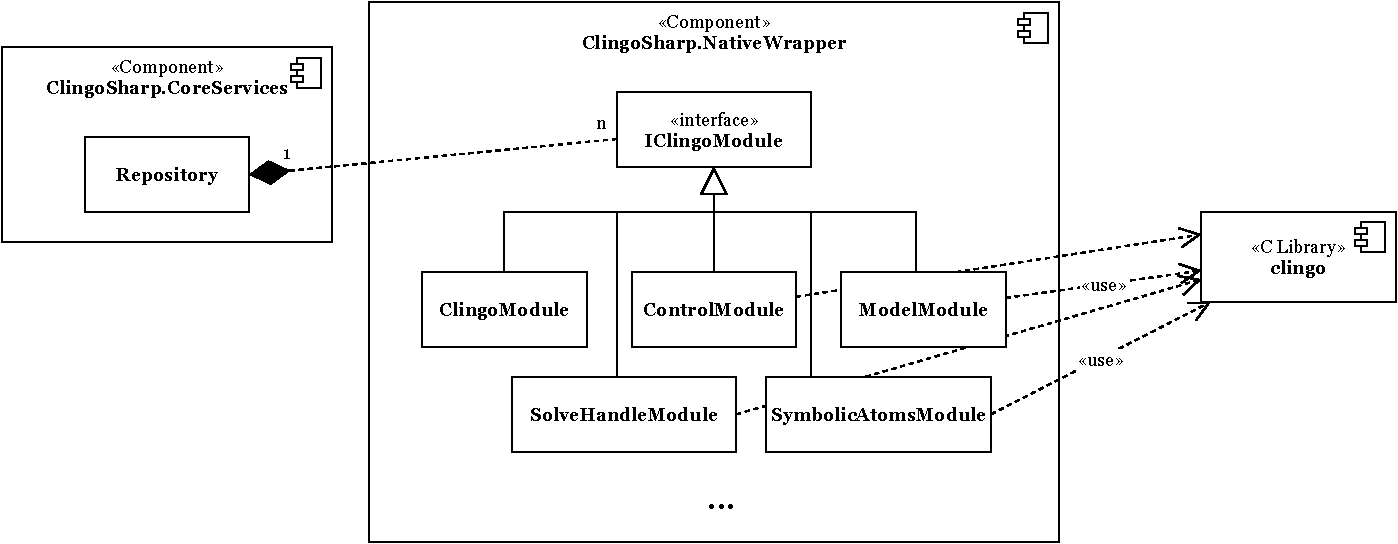
\includegraphics[width=\textwidth]{images/repository}
	\caption{Arquitectura de ClingoSharp}
	\label{fig:clingosharp-repository}
\end{figure}

En el caso del componente \texttt{ClingoSharp.CoreService}, este implementa la clase \texttt{Repository}, que contiene una composición de cada uno de los módulos. Esto es debido a que antes se pasa a memoria la biblioteca en Clingo, haciendo uso de los servicios disponibles en cada sistema operativo y de .NET Framework. Una vez realizada la carga en memoria, se procede a cargar dinamicamente cada uno de los módulos marcados con la interfaz \texttt{IClingoModule} del componente \textit{ClingoSharp.NativeWrapper}, y que finalmente son expuestos por nuestro repositorio.

En la Figura \ref{fig:clingosharp} se muestran las dependencias de cada uno de los distintos módulos. A pesar de lo complicado que parece, la arquitectura en repositorio nos permite abstraer la parte de enlazado de nuestro programa con la biblioteca nativa de Clingo, del enlazado de cada uno de los diferentes punto de control de la biblioteca, además de exponer una API limpia de Clingo en C\#. Otro punto a favor de esta arquitectura es que también actúa como wrapper, permitiendo cambiar entre distintas versiones de la biblioteca nativa de Clingo sin cambiar nuestro código, así como de implementar otra biblioteca de Aswer Set Programming en C\#.

\begin{figure}[!h]
	\centering
	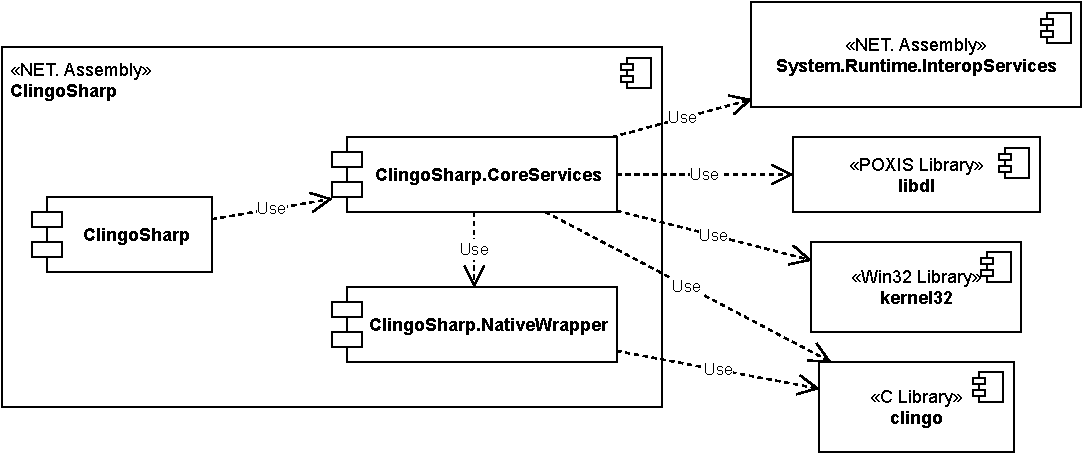
\includegraphics[width=\textwidth]{images/clingosharp}
	\caption{Dependencias de ClingoSharp}
	\label{fig:clingosharp}
\end{figure}

Para finalizar, cabe destacar que cada una de las capas (IndustryLP y ClingoSharp) se ejecuta en paralelo, pudiendo el primero enviar mensajes a ClingoSharp sin causar que la interfaz se congele, ademas de servir como recolector de errores que se puedan originar en nuestro programa lógico sin afectar a \cities.
	\cleardoublepage
	
	%\chapter{Evaluación}
	%\label{evaluation}
	%En este capítulo se analizará los resultados obtenidos en el proceso de evaluación del sistema. Para la planificación de las pruebas se ha optado por el uso de una herramienta de integración continua en donde se corren tanto pruebas de unidad a las partes del modelo de la interfaz gráfica, así como a los distintos módulos de los programas lógicos. \\

Además se ha usado un programa escrito en C\# para la ejecución de pruebas de rendimiento o \textit{benchmarks} el cual solo usa el módulo clingo para evitar el uso de la interfaz gráfica. En todas estas pruebas se ha añadido a las pruebas la restricción de que el cómputo del mapa solo puede durar como máximo cinco minutos, matando el proceso en caso de superar este tiempo y pasando a la siguiente prueba. Con esto podemos indicar cuales son las configuraciones que dan una experiencia pobre al usuario. \\

A continuación se describen los resultados obtenidos de estas pruebas de rendimiento con distintos parámetros. \\

\section{Tamaño de los mapas}

TODO
	%\cleardoublepage
	
	\hypertarget{conclusions}{\chapter{Conclusiones}}
	\label{conclusions}
	En este proyecto se ha enmarcado en el área de la representación del conocimiento. En especial, hemos construido una herramienta declarativa con la que elaborar, mediante programación lógica, polígonos industriales. Esto nos ha permitido crear una herramienta que, en manos de un experto, puede automatizar procesos de construcción de nuevos entornos industriales. Además, al apoyarnos en una herramienta de simulación como es \cities, podemos simular distintas carga de tráfico, una vez generado el polígono. \\

Como ya hemos comentado, gracias al uso de una herramienta declarativa, y de que la parte de definición del programa lógico es externo al algoritmo de búsqueda de modelos estables; un experto en construcción urbanística o de diseño de plantas industriales podría modificar o añadir reglas a su antojo para que la herramienta se adaptara lo máximo posible a su forma de trabajar. Además puede servir como base de datos en un futuro para guardar el tipo de estilo de expertos. \\

Otra parte importante de este trabajo es la construcción del binding de Clingo para el lenguaje de programación C\#. Aún no siendo el objetivo de este proyecto, al ser una biblioteca creada de forma desacoplada del proyecto principal, permite que más personas puedan usar las herramientas de Clingo, en este caso en proyectos creados para .NET. Esto permite una difusión mayor de la programación lógica, y en concreto de Answer Set Programming, para sistemas en los que posiblemente no se hubiera planteado hasta ahora como solución. \\

Para finalizar, este trabajo nos ha permitido ver como funciona un motor de videojuegos tan importante como lo es Unity, y en concreto como incorporar nuevas funcionalidades para un software que su fabricante no tenía pensado hasta ahora. Esto puede servir de gran ayuda para personas que quieran expandir su forma de jugar con un videojuego, además de servir de ejemplo y documentación para gente que esté pensando en entrar en el mundo del desarrollo de videojuegos.

\section{Trabajo futuro}

Con la finalización de este trabajo, se pueden sugerir diferentes líneas de trabajo futuro:

\begin{itemize}
	\item Permitir la generación de edificios de DLCs de \cities como \textit{Industries} o \textit{Sunset Harbor}, añadiendo las mecánicas de procesado de recursos. Además se podría incluir la generación de zonas de aparcamiento, parques y zonas verdes.
	\item Añadir más funcionalidades que nos permite clingo, como reglas de minimización y/o maximización, que permitan crear problemas de optimización a la hora de generar polígonos industriales. Además se podría añadir pesos a las reglas para permitir una generación más personalizada en función de lo que nos comente un experto sobre la construcción de polígonos industriales.
	\item Añadir reglas que permitan también la generación de las topologías de carreteras, pudiendo definir de forma declarativa las distribuciones e incluso unificando el proceso de generación.
	\item Mejorar la usabilidad de la herramienta, permitiendo marcar zonas a mano alzada o con distintas zonas y que tengan en cuenta el terreno. Además se podría incluir nuevas opciones para indicar, por ejemplo, la temática de los edificios a construir o prohibir la generación de un tipo concreto de edificio.
	\item Añadir información externa a la zona a construir, pudiendo unir de forma automática a autopistas o favoreciendo la conexión con zonas ya construidas.
\end{itemize}
	\cleardoublepage
	
	\listoftables
	\cleardoublepage
	
	\listoffigures
	\cleardoublepage
	
	\clearpage
	
	% ------- Appendices -------
	\appendix
	\addcontentsline{toc}{chapter}{Apéndices}
	\label{appendices}
	
	%\chapter{Diagramas}
	%\label{diagrams}
	%\input{tex/diagrams}
	%\cleardoublepage
	
	\hypertarget{manual}{\chapter{Manual de uso}}
	\label{manual}
	En esta sección mostraremos un pequeño manual de uso del mod creado para \cities, así como su instalación.

\section{Instalación}

Para proceder a instalar el mod, necesitaremos una cuenta de \href{https://store.steampowered.com/}{Steam}. Una vez creada, y habiendo comprado e instalado \cities en Steam, vamos a la WorkShop de \cities y buscamos \textit{IndustryLP}. Deberíamos de encontrar una entrada al mod que aparece en la Figura \ref{fig:mod}. \\

\begin{figure}[h]
	\centering
	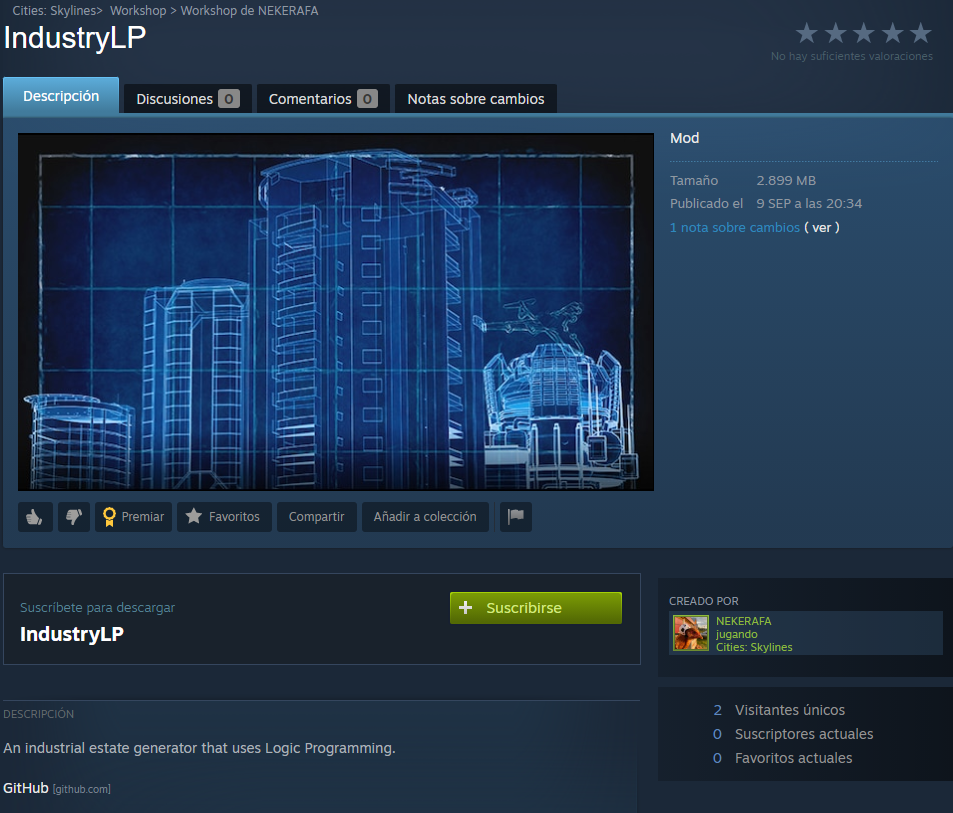
\includegraphics[width=\textwidth]{images/workshop}
	\caption{Página web del IndustryLP en la WorkShop de \cities.}
	\label{fig:mod}
\end{figure}

Una vez en la web del mod, solo tenemos que pulsar en el botón \texttt{Subscribe} para que la aplicación de escritorio instale los archivos necesario para ejecutar el mod.

\section{Uso}

Una vez subscritos, podemos ejecutar \cities. Para habilitar el mod, tenemos que entrar en el menú \texttt{Content Manager}, e ir a la sección \texttt{Mods}. Allí podremos buscar \textit{IndustryLP} y activarlo seleccionando el checkbox con la etiqueta \texttt{On / Off}, tal y como se muestra en la Figura \ref{fig:options}. \\

\begin{figure}[h]
	\centering
	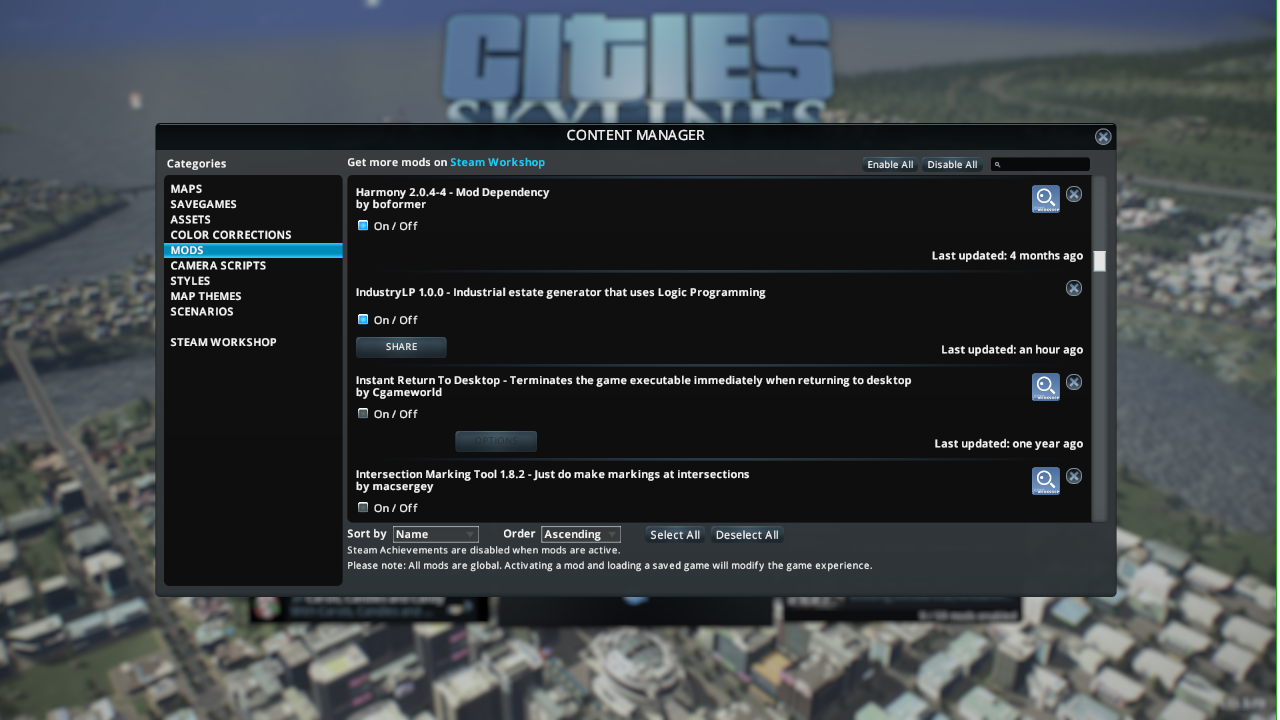
\includegraphics[width=\textwidth]{images/options}
	\caption{Activación de IndustryLP en \cities.}
	\label{fig:options}
\end{figure}

Con el mod activado, podemos empezar una nueva partida. Se nos activará un nuevo icono que permitirá lanzar el menú de la Figura \ref{fig:tool}. En el destacamos varias cosas:

\begin{figure}[h]
	\centering
	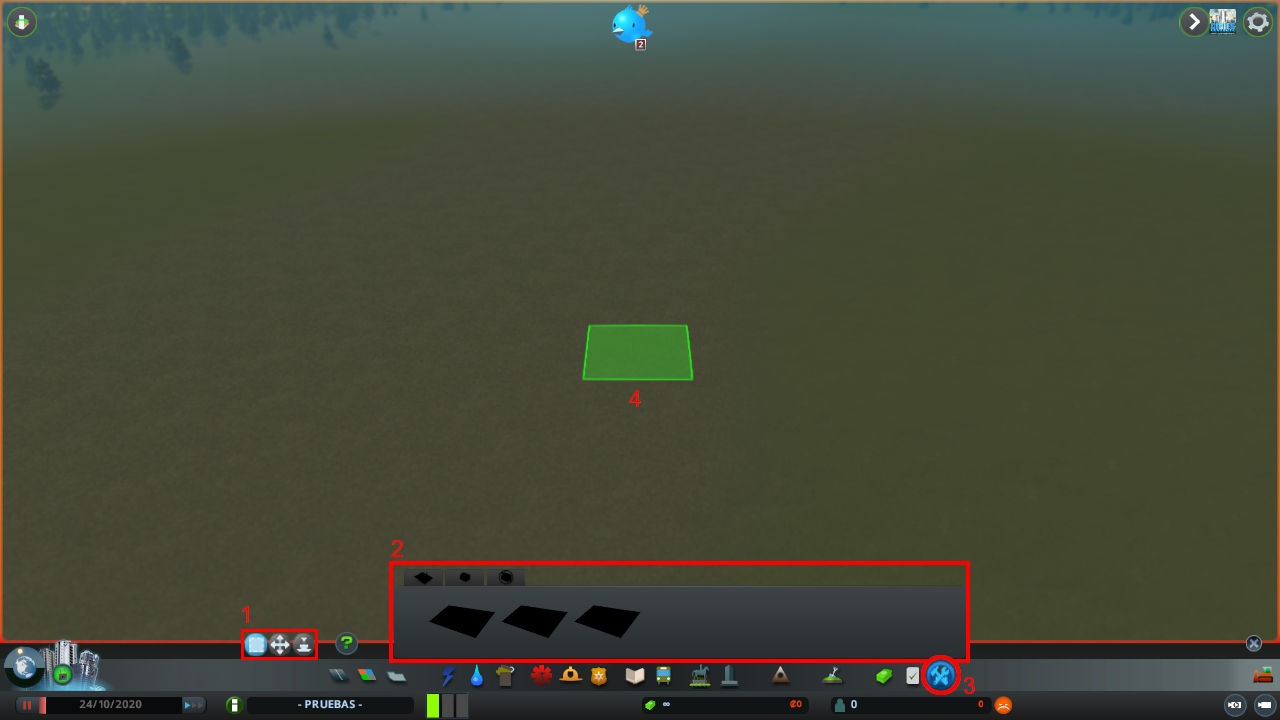
\includegraphics[width=\textwidth]{images/tool}
	\caption{Interfaz de IndustryLP.}
	\label{fig:tool}
\end{figure}

\begin{enumerate}
    \item \textbf{Acciones de la herramienta:} Se muestran tres iconos: Definir región, mover región y generar soluciones.
    \item \textbf{Panel de opciones:} En el podremos elegir las distribuciones predefinidas, así como definir preferencias y restricciones de edificios.
    \item Icono principal del mod.
    \item Cursor.
\end{enumerate}

\subsection{Definir región}

Cuando pulsamos en el icono de la acción \textbf{Definir región} se nos activará un cursor con un cuadrado verde en el mapa. Si mantenemos pulsado en una región, este cuadrado cambiará a una selección de color naranja. \\

Una vez terminada la selección, se nos mostrará la selección de color blanco, con cuatro puntos verdes en cada arista y uno en el centro, tal y como se muestra en la Figura \ref{fig:selection}. Si el tamaño no fuera el suficiente, esta selección será roja, y al dejar de pulsar se desmarcará al no ser válida, como recogemos en la Figura \ref{fig:bad-selection}.

\begin{figure}[h]
	\centering
	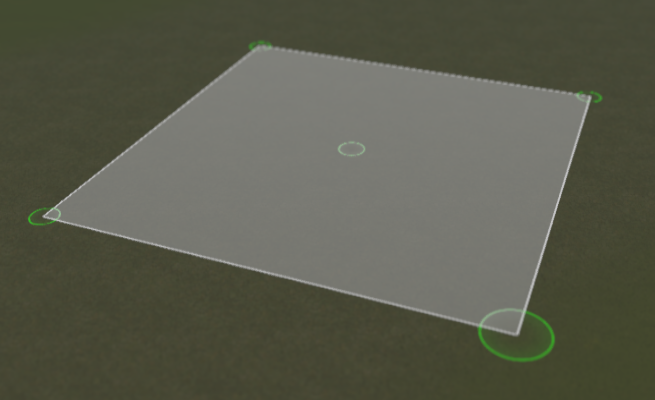
\includegraphics[width=0.5\textwidth]{images/selection}
	\caption{Región correctamente seleccionada.}
	\label{fig:selection}
\end{figure}

\begin{figure}[h]
	\centering
	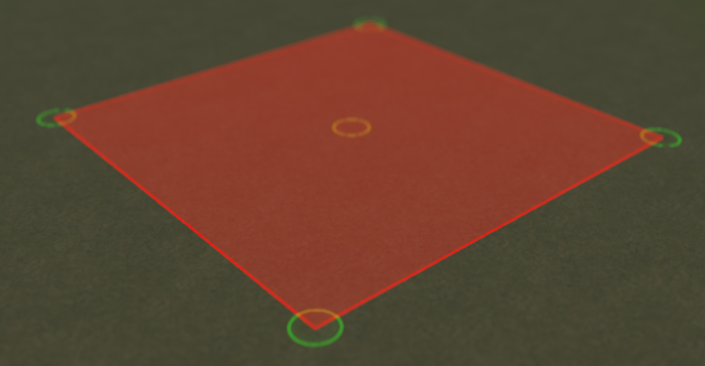
\includegraphics[width=0.5\textwidth]{images/bad-selection}
	\caption{Región con tamaño insuficiente.}
	\label{fig:bad-selection}
\end{figure}

\subsection{Mover región}

Una vez realizada una selección, se nos habilitará la acción de \textbf{Mover región} que nos mostrará la selección de la misma forma que en la Figura \ref{fig:selection}. \\

Esta acción nos permitirá modificar el la posición de cada uno de sus vértices verdes, así como mover la selección pulsando en el círculo central de la selección, y rotarla. Para rotarla tendremos que pulsar el botón derecho del ratón en cualquier parte del mapa, y sin soltarlo, moverlo.

\subsection{Distribuciones del terreno}

Cuando tengamos una selección hecha, se nos habilitará en el panel de opciones la pestaña de \textit{Distribuciones} (Figura \ref{fig:distributions-panel}). Al pinchar en cualquiera de las opciones, IndustryLP calculará que distribución hacer dentro de la selección. Este proceso puede tardar escasos segundos, los suficientes para que \cities se congele si la selección es muy grande.

\begin{figure}[h]
	\centering
	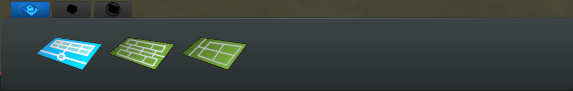
\includegraphics[width=\textwidth]{images/distributions}
	\caption{Panel con la lista de distribuciones.}
	\label{fig:distributions-panel}
\end{figure}

\subsection{Añadir preferencias / restricciones}
\label{subsec:pref}

Con la distribución de caminos generada, se nos habilitará las pestañas de \textit{Preferencias} y \textit{Restricciones}, tal y como se muestra en la Figura \ref{fig:preferences}. En ellas, podremos seleccionar un edificio de industria que viene incluido en \cities y, o indicar su posición en el caso de una preferencia, o indicar a IndustryLP que no genere ese edificio en una posición dada. \\

\begin{figure}[h]
	\centering
	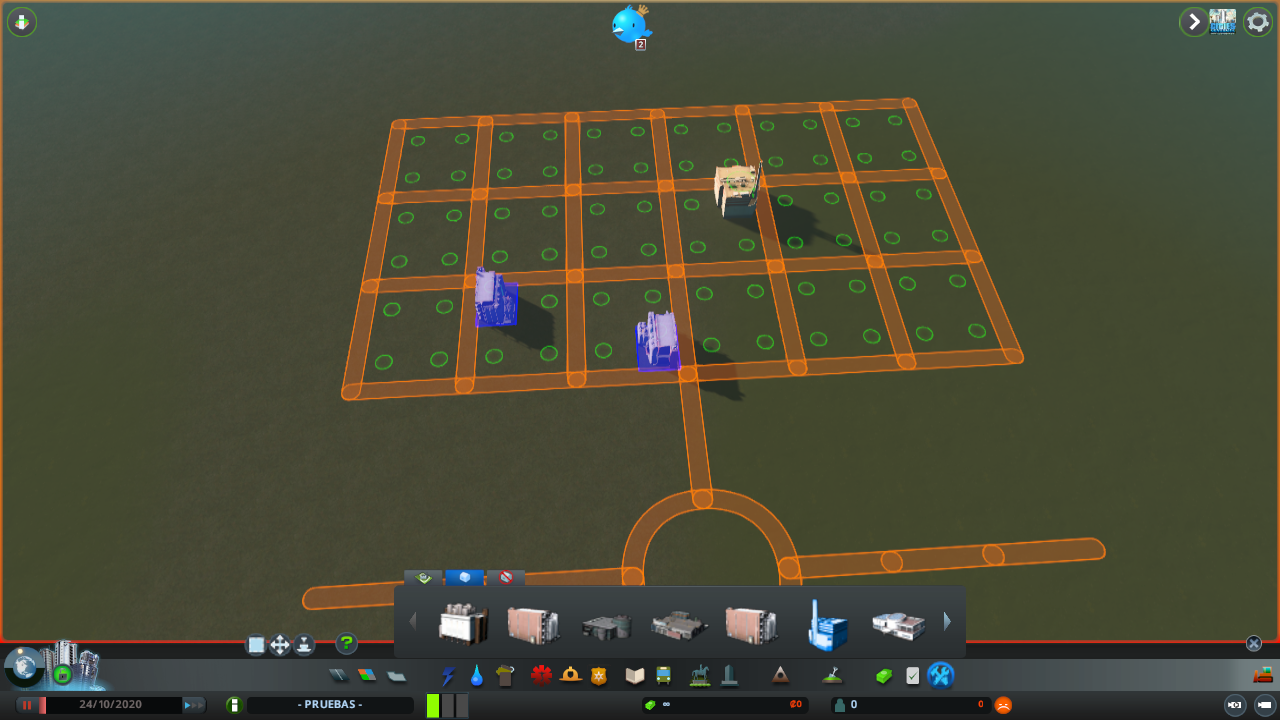
\includegraphics[width=\textwidth]{images/preferences}
	\caption{Varias preferencias de edificios posicionadas en la selección hecha.}
	\label{fig:preferences}
\end{figure}

Una vez seleccionado un edificio, IndustryLP pasará a la acción de añadir preferencia/restricción, y junto a la distribución de carreteras nos saldrán puntos verdes en donde fijar la posición del edificio. Cuando estemos modificando preferencias, los edificios ya establecidos se nos mostrarán junto con el área edificable en color azul. En el caso de que estemos modificando restricciones, nos aparecerán solo los edificios indicados como restricción. \\

Si por un casual queremos borrar una selección, tendremos que pulsar el botón derecho del ratón cerca de una posición dada. \\

Una cosa a tener en cuenta es que, si pusiéramos un mismo edificio como restricción y preferencia, el programa no generaría ninguna solución. Esto es debido a que el sistema lógico no encuentra una solución que satisfaga las dos reglas a la vez.

\subsection{Generación de industrias}

Cuando tengamos una distribución generada, y opcionalmente marcadas las preferencias y restricciones, se nos habilitará el icono de la acción de \textbf{Generar soluciones}. Si la activamos, se nos mostrará el diálogo de la Figura \ref{fig:dialog} con varias opciones para modificar.

\begin{figure}[h]
	\centering
	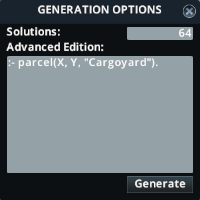
\includegraphics[width=0.4\textwidth]{images/dialog}
	\caption{Opciones de la generación.}
	\label{fig:dialog}
\end{figure}

\begin{enumerate}
    \item \textbf{Soluciones:} número de soluciones que el sistema deberá generar. 0 para generar todas las posibles.
    \item \textbf{Edición avanzada:} Nos permitirá incorporar reglas en el formato \textit{ASP Core 2}, que es el formato con el que trabaja la herramienta \clingo.
    
    Existen algunas reglas predefinidas de distancia y vecinos con las que podemos trabajar de forma inmediata. Otro tipo de reglas las deberemos escribir en este campo o crear un archivo de programa lógico, tal y como se expone en la Sección \ref{subsec:logic-files}.
\end{enumerate}

Si pulsamos en el botón \textbf{Generate}, el panel de opciones se nos modificará a como aparece en la Figura \ref{fig:solutions}. En esta nueva interfaz podremos destacar varias zonas:

\begin{figure}[h]
	\centering
	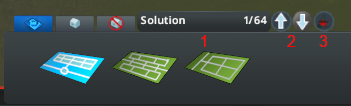
\includegraphics[width=0.6\textwidth]{images/solutions}
	\caption{Menú de selección de solución.}
	\label{fig:solutions}
\end{figure}

\begin{enumerate}
    \item Panel con el índice de la solución actual / soluciones totales encontradas.
    \item Botones para ir a la solución anterior / posterior.
    \item Construir solución.
\end{enumerate}

El resultado de la generación de la solución actual se mostrará en la selección actualmente hecha. Cuando estemos convencidos con una solución, podemos pulsar el botón de construir solución y todo se construirá dentro de \cities. \\

En el caso de que el problema sea insatisfactible, ya sea al indicar reglas incompatibles de la forma en la que se comenta al final de la Sección \ref{subsec:pref}, o al añadir reglas en la edición avanzada; se nos mostrará la interfaz de la misma forma que en la figura \ref{fig:unsat-solution}.

\begin{figure}[h]
	\centering
	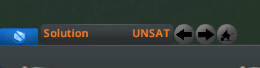
\includegraphics[width=0.4\textwidth]{images/unsat-solution}
	\caption{Ejemplo de programa insatisfactible.}
	\label{fig:unsat-solution}
\end{figure}

\subsection{Edición avanzada}
\label{subsec:logic-files}

Otra opción para hacer una edición avanzada, y además de poder modificar la generación de IndustryLP con nuevas reglas es modificar los archivos con los programas lógicos que IndustryLP carga en cada generación. Si el mod ha sido instalado mediante Steam, estos archivos se localizarán en la ruta \texttt{Program Files (x86) / Steam / SteamApps / WorkShop / Content / 255710 / 2597556943 / logic\_program }. \\

Cualquier archivo que se cree en esta carpeta con la extensión \texttt{.lp} será cargado dentro del proceso de Clingo, por lo que el usuario puede crear archivos con programas lógicos a voluntad sin tener que recompilar el mod, y pudiendo persistir estos programas entre generación y generación. \\

En el Apéndice \ref{asp} se explica de forma detallada el contenido de los distintos archivos creados por defecto y que sirven de documentación para la ampliación de reglas.
	\cleardoublepage
	
	%\chapter{Información de Lua}
	%\label{lua}
	%\input{tex/lua}
	%\cleardoublepage
	
	\clearpage
	
	% ------- Biliography -------
	\bibliographystyle{IEEEtran-spanish}
	\bibliography{bib/references}
	\addcontentsline{toc}{chapter}{B. Bibliografía}
	\label{bibliography}
\end{document}